\title{ROBustness In Network (\pkg{robin}): an R Package for Comparison and Validation of Communities }

\author{by Valeria Policastro, Dario Righelli, Annamaria Carissimo, Luisa Cutillo and Italia De Feis}

\maketitle

\abstract{In network analysis, many community detection algorithms have been developed. However, their implementation leaves unaddressed the question of the statistical validation of the results. Here, we present \CRANpkg{robin} (ROBustness In Network), an R package to assess the robustness of the community structure of a network found by one or more methods to give indications about their reliability. The procedure initially detects if the community structure found by a set of algorithms is statistically significant and then compares two selected detection algorithms on the same graph to choose the one that better fits the network of interest. We demonstrate the use of our package on the American College Football benchmark dataset.
}


\section{Introduction} \label{sec:intro}

Over the last twenty years, network science has become a strategic field of research thanks to the strong development of high-performance computing technologies. The activity and interaction of thousands of elements can now be measured simultaneously, allowing us to model cellular networks, social networks, communication networks, power grids, and trade networks, to cite a few examples. Different types of data will produce different types of networks in terms of structure, connectivity, and complexity. In the study of complex networks, a network is said to have a community structure if the nodes are densely connected within groups but sparsely connected between them \citep{GirvanNewman:2002}. 
The inference of the community structure of a network is an important task. Communities allow us to create a large-scale map of a network since individual communities act like meta-nodes in the network, which makes its study easier. Moreover, community detection can predict missing links and identify false links in the network. Despite its difficulty, a huge number of methods for community detection have been developed to deal with different size complexity and made available to the scientific community by open-source software packages. In this paper, we will address a specific question: are the detected communities significant, or are they a result of chance only due to the positions of edges in the network?

An important answer to this question is the Order Statistics Local Optimisation Method ($OSLOM$, \url{http://www.oslom.org/}) presented in \cite{Lancichinetti_et_al:2011}. $OSLOM$ introduces an iterative technique based on the local optimization of a fitness function, the C-score \citep{Lancichinetti_et_al:2010}, expressing the statistical significance of a cluster with respect to random fluctuations. The significance is evaluated by fixing a threshold parameter P a priori.

Another interesting approach is the Extraction of Statistically Significant Communities ($ESSC$, \url{https://github.com/jdwilson4/ESSC}) technique proposed in \cite{Wilson_et_al:2014}. The algorithm is iterative and identifies statistically stable communities measuring the significance of connections between a single vertex and a set of vertices in undirected networks under the configuration model \citep{Bender_Canfield:1978} used as the null hypothesis. The method employs multiple testing and false discovery rate control to update the candidate community. 

\cite{Kojaku_Masuda:2018} introduced the QStest (\url{https://github.com/skojaku/qstest/}), a method to statistically test the significance of individual communities in a given network. Their algorithm works with different detection algorithms using a quality function that is consistent with the one used in community detection and takes into account the dependence of the quality function value on the community size. QStest assesses the statistical significance under the configuration model too.

Very recently, \cite{He_et_al:2020} suggested the Detecting statistically Significant Communities (DSC) method, a significance-based community detection algorithm that uses a tight upper bound on the p-value under the configuration model coupled with an iterative local search method.

OSLOM, ESSC, and DSC assess the statistical significance of every single community analytically while QStest adopts the sampling method to calculate the p-value of a given community.
Moreover, all of them detect statistically significant communities under the configuration model, and only QStest is independent of the detection algorithm.

We present \pkg{robin} (ROBustness In Network), an R/CRAN package whose purpose is to give clear indications about the reliability of one or more community detection algorithms understudy, analyzing their robustness with respect to random perturbations. The idea behind \pkg{robin} is that if a partition is significant, it will be recovered even if the structure of the graph is modified. Alternatively, if the partition is not significant, minimal modifications of the graph will be sufficient to change it. \pkg{robin} is inspired by the concept presented by \cite{Carissimo_et_al:2018}, who studied the stability of the recovered partition against random perturbations of the original graph structure using tools from Functional Data Analysis (FDA). 

\pkg{robin} provides the best choice among the variety of the existing methods for the network of interest. It is based on a procedure that gives the opportunity to use the community detection techniques implemented in the igraph package \cite{Csardi:2019} while providing the user with the possibility to include other community detection algorithms.
\pkg{robin} initially detects if the community structure found by some algorithms is statistically significant, then it compares the different selected detection algorithms on the same network.
\pkg{robin} assumes undirected graphs without loops and multiple edges.


\pkg{robin} looks at the global stability of the detected partition and not of single communities but accepts any detection algorithm and any random model, and these aspects differentiate it from OSLOM, ESSC, DSC, and QStest.
Unlike other studies that treat the comparison between algorithms in a theoretical way, such as \cite{Yang_et_al:2016}, \pkg{robin} aims to give a practical answer to such a comparison that can vary with the network of interest.


\section{The model} \label{sec:model}


\pkg{robin} implements a methodology that examines the stability of the recovered partition by one or more algorithms. The methodology is useful for two purposes: to detect if the community structure found is statistically significant or is a result of chance; to choose the detection algorithm that better fits the network under study. These are implemented following two different workflows.\hfill \break



The \textbf{\emph{\underline{first workflow}}} tests the stability of the partitions found by a single community detection algorithm against random perturbations of the original graph structure. To address this issue, we specify a perturbation strategy (see subsection \textbf{\ztitleref{sec:Perturbation strategy}}) and a null model to build some procedures based on a prefixed stability measure (see subsection \textbf{\ztitleref{sec:Stability measure}}).
Given:
\begin{itemize}
    \item a network of interest $g1$
    \item its corresponding null random model $g2$
    \item a Detection Algorithm (DA)
    \item a stability measure (M)
\end{itemize}  
Our process builds two curves as functions of the perturbation level $p$, as shown in Figure \ref{fig:PlotExample}, and tests their similarity by two types of functional statistical tests (see subsection \textbf{\ztitleref{sec:Statistical Tests}}).

\begin{figure}[!h]
\centering
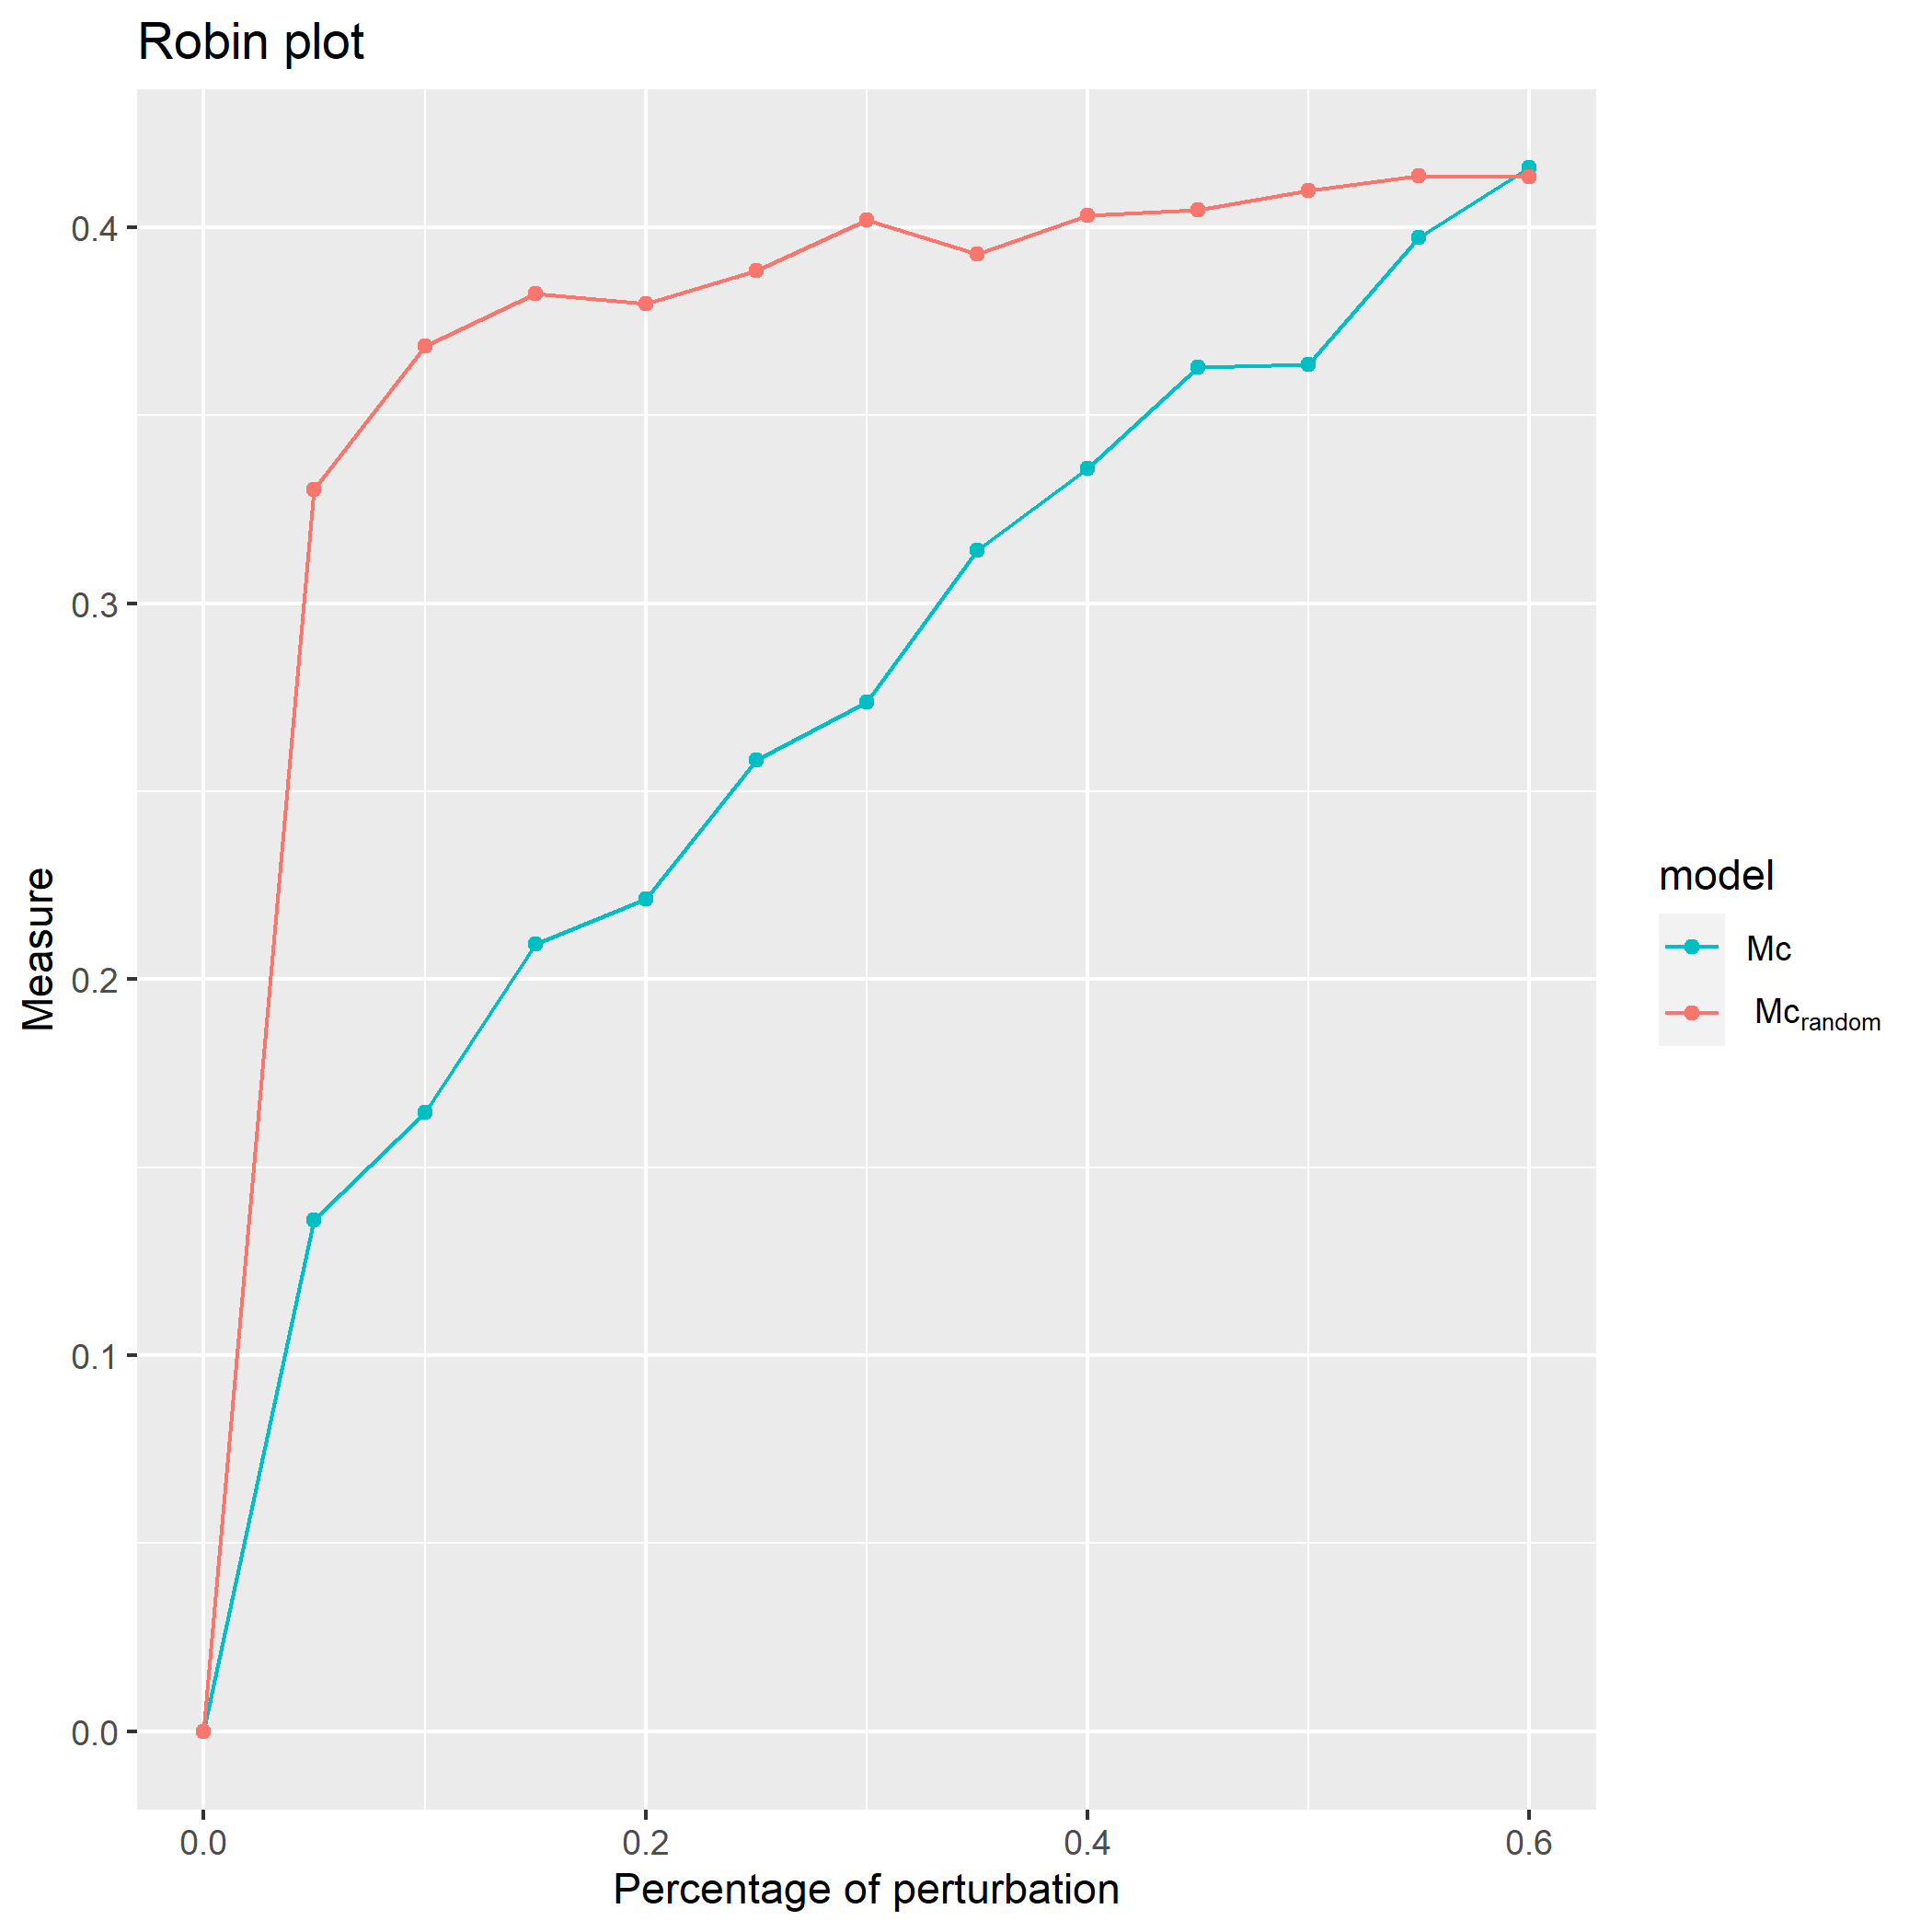
\includegraphics[width=.5\textwidth, height=6cm]{PlotExample.png}
\caption{\label{fig:PlotExample} Example of $Mc_{random}$ and $Mc$ curves generated by an M stability measure}
\end{figure}


The first curve $Mc$ is obtained by computing M between the partition of the original network $g1$ and the partition of a different perturbed version of $g1$. The second curve $Mc_{random}$ is obtained by computing
M between the partition of a null random network  $g2$ and the partition of a different perturbed version of  $g2$. 



The comparison between the two M curves enables us to reconsider the problem regarding the significance of the retrieved community structure in the context of stability/robustness of the recovered partition against perturbations. 
The basic idea is that if small changes in the network cause a completely different grouping of the data, the detected communities are not reliable. 
For a better understanding of this point, we refer the reader to the paper \cite{Carissimo_et_al:2018} where the methodology was developed. 


The choice of the null model plays a key role because we would expect it to reproduce the same structure of the real network but with completely random edges.
For this reason, \pkg{robin} offers two possibilities: a degree preserving randomization by using the \code{rewire} function of the  \CRANpkg{igraph} package or a model chosen by the user. 



The degree preserving randomization, i.e., Configuration Model (CM), is a model able to capture and preserve strongly heterogeneous degree distributions often encountered in real network data sets and is the standard null model for empirical patterns. Nevertheless, it can happen that it is not sufficient to preserve only the degree of the graph understudy, so \pkg{robin} allows the user to include their own null model. 



In section \textbf{\ztitleref{sec:example}}, we explore the $dk$ null random model provided in 
\cite{Orsini_et_al:2015}, whose code is available at \url{https://github.com/polcolomer/RandNetGen} as a possible alternative to CM.
The {\it dk}-series model generates a random graph preserving the global organization of the original network at various increasing levels of details chosen by the user via the setting of the parameter $d$. More precisely, the {\it dk}-series is a converging series of properties that characterize the local network structure at an increasing level of detail and define a corresponding series of null models or random graph ensembles. 
Increasing values of $d$ capture progressively more properties of the network:  {\it dk} 1 is equivalent to randomizing the network fixing only the degree sequence, {\it dk} 2 fixes additionally the degree correlations, {\it dk} 2.1 fixes also the clustering coefficient, and {\it dk} 2.5 the full clustering spectrum.




The first workflow is summarised as follows (see Figure \ref{fig:Flowchart1}):

\begin{enumerate}
\item find a partition $C_1$ for the real network and a partition $C_2$ for the null network, 
\item perturb both networks, 
\item retrieve two new partitions $C_{1(p)}$ and $C_{2(p)}$, 
\item calculate two clustering distances (for the real network and the null network) between the original partitions and the ones obtained from the perturbed network as:
\begin{equation}
M\left(C_{1\left(p\right)},C_1\right) \quad \mathrm{and} \quad M\left(C_{2\left(p\right)},C_2\right)  
\end{equation}
\end{enumerate}
Steps 2) - 4) are computed at different perturbation levels $p \in [0:0.05:0.6]$ to create two curves, one for the real network and one for the null model, then their similarity is tested by two functional statistical tests described in subsection \textbf{\ztitleref{sec:Statistical Tests}}.

\begin{figure}[h!]
\centering
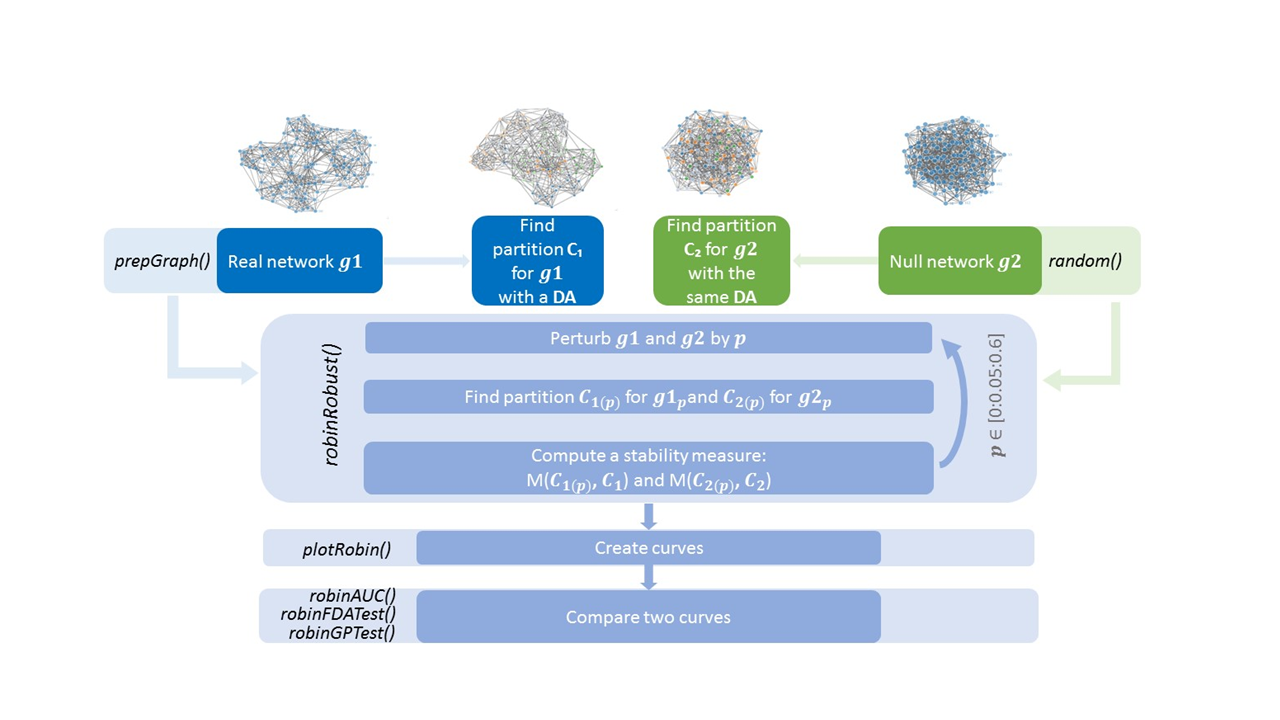
\includegraphics[width=.9\textwidth, height=9cm]{Figure1.png}
\caption{\label{fig:Flowchart1} Workflow to test the goodness of a community detection algorithm.}
\end{figure}

This procedure allows the filtering of the detection algorithms according to their performance. Moreover, the selected ones can be compared using the second workflow.\hfill \break



The \textbf{\emph{\underline{second workflow}}} helps to choose among different community detection algorithms the one that best fits the network of interest, comparing their robustness two at a time.
More precisely, the technique (see Figure \ref{fig:Flowchart2}): 
\begin{enumerate}
\item find two partitions $C_1$ and $C_2$ inferred by two different algorithms on the network under study, 
\item perturb the network creating a new one, 
\item retrieve two new partitions $C_{1(p)}$ and $C_{2(p)}$,
\item evaluate $M\left(C_{1\left(p\right)},C_1\right)$  and $M\left(C_{2\left(p\right)},C_2\right)$.  
\end{enumerate}
Steps 2) - 4) are repeated at different perturbation levels $p \in [0:0.05:0.6]$ to create two curves and then their similarity is tested.

\begin{figure}[h!]
\centering
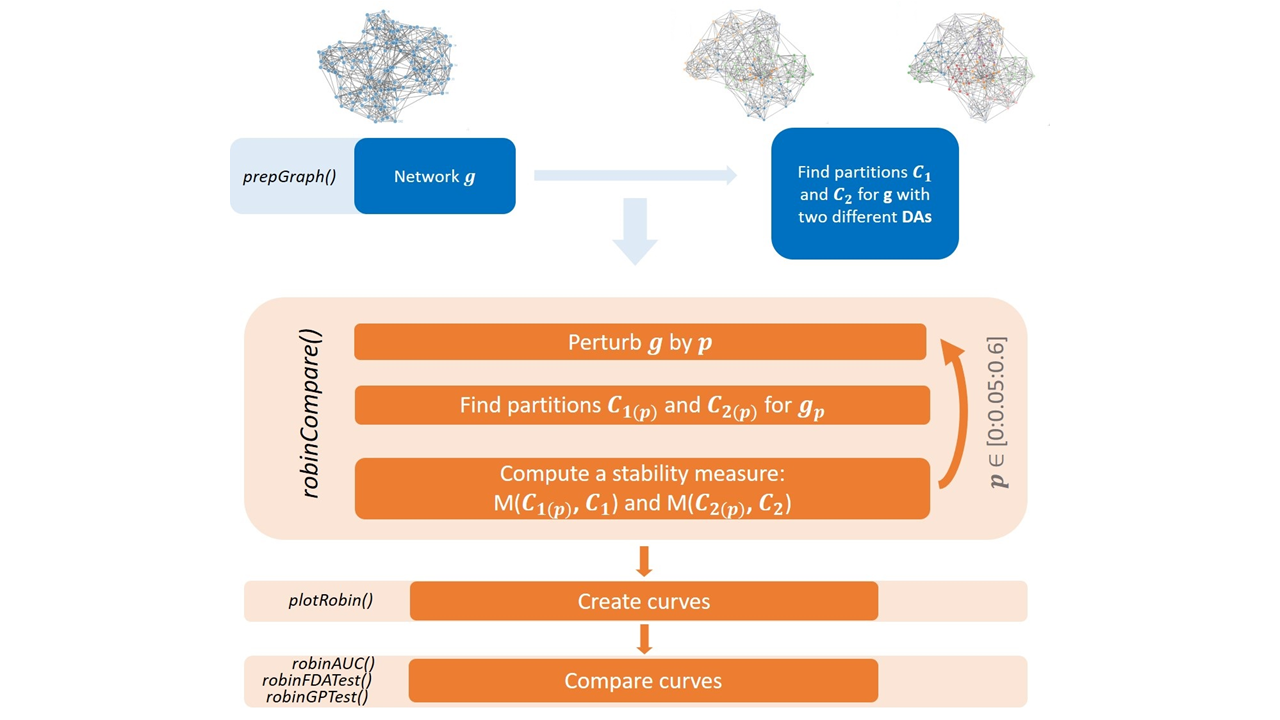
\includegraphics[width=.9\textwidth, height=9cm]{Figure2.png}
\caption{\label{fig:Flowchart2} Workflow to compare two different community detection algorithms.}
\end{figure}

\subsection{Perturbation strategy}\zlabel{sec:Perturbation strategy}
The perturbed network has been restricted to have the same number of vertices and edges as the original unperturbed network. Therefore, only the positions of the edges are changed. It is expected that if a community structure is robust, it should be stable under small perturbations of the edges. This is because perturbing the network edges by a small amount will imply just a small percentage of nodes to be moved in different communities; on the other hand, perturbing a high percentage of the edges in the network will produce random clusters. Note that zero perturbation $p=0$ corresponds to the original graph while a maximal perturbation level $p=1$ will correspond to the random graph. Therefore, in \pkg{robin}, the perturbation of a network preserves the degree distribution of the original network. 

Two different procedures for the perturbation strategy are implemented, namely independent and dependent types. The independent strategy introduces a percentage $p$ of perturbation in the original graph at each iteration, for $p=0,\dots,p_{max}$. Whereas the dependent procedure introduces $5\%$ of perturbation at each iteration on the previous perturbed graph, starting from the original network, until $p_{max}$ of the graph's edges are perturbed. In the implementation of the perturbation strategy, we set up $p_{max}=0.6$, because the structure of the network becomes random if we perturb more than $50\%$ of the edges. 

In particular, we noticed that the greatest modification of the network structure happens for a perturbation level between $30\%$ and $40\%$ if a network is robust, while it happens at very low perturbation levels if the network is not robust. 

We stress again that the M curve for a network with a strong structure grows rapidly (perturbation level between 0$\%$ and 40$\%$) then levels off when $50\%<p<100\%$.

Moreover, the choice $p_{max}=0.6$ reduces computational time and shows more clearly the differences between the curves.


Varying the percentage of perturbation, many graphs are generated and compared by means of the stability measure chosen. For each perturbation level, we generated 10 perturbed graphs and calculated the stability measure. From each of these graphs, we generated 9 more by rewiring an additional $1\%$ of the edges. Therefore, the procedure generates 100 graphs with the respective stability measures for each level of $p$ and gives as output the mean of the stability measure for every 10 graphs generated.

\subsection{Stability measure}\zlabel{sec:Stability measure}	
The procedure we implemented is based on four different stability measures:
\begin{itemize}
\item	 the Variation of Information (VI) proposed by \cite{Meila:2007}, 
\item the Normalized Mutual Information (NMI) measure proposed by \cite{Danon_et_al:2005},
\item the split-join distance of \cite{vanDongen:2000},
\item the Adjusted Rand Index (ARI) by \cite{HubertArabie:1985}.
\end{itemize}
VI measures the amount of information lost and gained in changing from one cluster to another, while split-join distance calculates the number of nodes that have to be exchanged to transform any of the two clusterings into the other; but for both of them, low values represent more similar clusters, and high values represent more different clusters. On the contrary, NMI and ARI are similarity measures, and therefore, lower values identify more different clusters and higher values more similar ones. To make all the measures comparable, we considered the 1-1 transformation for the NMI and the ARI since they vary between $[0,1]$ as: 
\begin{align}
f\left(X\right)=1-X  
\end{align}
Only two of the four proposed stability measures, i.e., split-join and VI, are distances. They differ in their dependency on the number of clusters K: while the VI distance grows logarithmically with K, the split-join metric grows with K toward the upper bound of 1. To make the four different stability measures comparable, we normalized VI and split-join between 0 and 1 (i.e., we divided the VI and the split-join by their maximum, respectively $\log\left(n\right)$ and $2n$, where n indicates the number of vertices in the graph).
	
\subsection{Statistical tests}\zlabel{sec:Statistical Tests}
\pkg{robin} allows different multiple statistical tests to check the differences between the real and the random curve or between the curves built from two different detection algorithms. 
The variation of $p$ from $0$ to $0.6$ induces an intrinsic order to the data structure as in temporal data. This lets $p$ assume, the same role as a time point in a temporal process, and as a consequence, we can use any suitable time series approach to compare our curves. In the following, we describe the use of two such approaches.

The first is a test based on the Gaussian Process regression (GP) described in \cite{KalaitzisLawrence_paper:2011}. In this paper, the authors use GP to compare treatment and control profiles in biological time-course experiments. The main idea is to test if two time series represent the same or two different temporal processes.
%testo colorato
A Gaussian process is a collection of random variables, any finite number of which have a joint Gaussian distribution and is completely specified by its mean function and its covariance function, see e.g., \cite{Rasmussen:2006}. Given the mean function $m\left(x\right)$ and the covariance function $k\left(x,x'\right)$ of a real process $f\left(x\right)$, we can write the GP as:
\begin{equation}
f\left(x\right) \sim \mathcal{GP}\left(m\left(x\right), k\left(x,x'\right)\right).
\end{equation}
The random variables $\mathbf{f}=\left(f\left(X_1\right),\dots,f\left(X_n\right)\right)^T$ represent the value of the function $f(x)$ at time locations $\left(X_i\right)_{i=1,\dots,n}$, being $f(x)$ the true trajectory/profile of the gene. Assuming $f(x)=\Phi(x)^T\mathbf{w}$, where $\Phi(x)$ are projection basis functions, with prior $\mathbf{w} \sim N(\mathbf{0},\sigma_{\mathbf{w}}^2\mathbf{I})$, we have
\begin{align}
&&m\left(x\right)=\Phi\left(x\right)^TE\left[\mathbf{w}\right]=0, \quad k\left(x,x'\right)=\sigma_{\mathbf{w}}^2\Phi\left(x\right)^T\Phi\left(x\right) \label{GPbayes_mean_cov}\\
&&f\left(x\right) \sim \mathcal{GP}\left(0,\sigma_{\mathbf{w}}^2\Phi\left(x\right)^T\Phi\left(x\right)\right).
\end{align} 
Since observations are noisy, i.e., $\mathbf{y}=\mathbf{\Phi w}+\pmb{\varepsilon}$, with $\mathbf{\Phi}=(\Phi(X_1)^T,\dots,\Phi(X_n)^T)$, assuming that the noise $\pmb{\varepsilon} \sim N(\mathbf{0},\sigma_n^2\mathbf{I})$ and using 
Eq. (\ref{GPbayes_mean_cov}), the marginal likelihood becomes:
\begin{align}
p(\mathbf{y} | \mathbf{x})=\frac{1}{\left(2\pi\right)^{n/2}\left|\mathbf{K_y}\right|^{1/2}}\mathrm{exp}\left(-\frac{1}{2}\mathbf{y}^t\mathbf{K_y}^{-1}\mathbf{y}\right), \label{GPmarginal}
\end{align}
with $\mathbf{K_y}=\sigma_{\mathbf{w}}^2\mathbf{\Phi}\mathbf{\Phi}^T+\sigma_n^2\mathbf{I}$.

In this framework, the hypothesis testing problem over the perturbation interval $[0,p_{max}]$ can be reformulated as:
\begin{equation}
H_0: \log_2  \frac{M_1\left(x\right)}{M_2\left(x\right)}  \sim GP\left(0,k\left(x,x'\right)\right)  \quad \mathrm{against} \quad H_1: \log_2  \frac{M_1\left(x\right)}{M_2\left(x\right)} \sim GP\left(m\left(x\right),k\left(x,x'\right)\right)  ,
\end{equation}
where $x$ represents the perturbation level.
To compare the two curves, \pkg{robin} uses the Bayes Factor (BF), which is approximated with a log-ratio of marginal likelihoods of two GPs, each one representing the hypothesis of differential (the profile has a significant underlying signal) and non-differential expression (there is no underlying signal in the profile, just random noise). 

The second test implemented is based on the Interval Testing Procedure (ITP) described in \cite{PiniVantini:2016}.
The ITP provides an interval-wise nonparametric functional testing and is not only able to assess the equality in distribution between functions, but also to underline specific differences. 
Indeed, users can see where are localized the differences between the two curves.
The Interval Testing Procedure is based on: 
\begin{enumerate}
\item Basis Expansion: functional data are projected on a functional basis (i.e. Fourier or B-splines expansion);
\item Interval-Wise Testing: statistical tests are performed on each interval of basis coefficients;
\item Multiple Correction: for each component of the basis expansion, an adjusted \textbf{\emph{p}}-value is computed from the \textbf{\emph{p}}-values of the tests performed in the previous step.
\end{enumerate}
In summary, GP provides a global answer on the dissimilarity of the two M curves, while ITP points out local changes between such curves. As a rule of thumb, we suggest initially using GP to flag a difference and then ITP to understand at which level of perturbation such a difference is locally significant.

We also provide a global method to quantify the differences between the curves when they are very close. This is based on the calculation of the area under the curves with a spline approach.

\section{Package structure} \zlabel{sec:package}	
\subsection{Installation}
Once in the R environment, it is possible to install and load the \pkg{robin} package with its dependencies, as follows:

\begin{example}
install.packages("robin")
\end{example}

The \pkg{robin} package includes as dependencies \pkg {igraph} \citep{Csardi:2019}, \CRANpkg{networkD3}  \citep{Allaire:2017},  \CRANpkg{ggplot2} \citep{Wickham:2019},  \CRANpkg{gridExtra} \citep{Auguie2017},  \CRANpkg{fdatest} \citep{PiniVantini:2015} , \BIOpkg{gprege} \citep{KalaitzisLawrence2011}, and  \CRANpkg{DescTools} \citep{Signorell2019} packages. All, except \pkg{gprege} which is a Bioconductor package, are automatically loaded with the command: 

\begin{example}
library(robin). 
\end{example}

To install the \pkg{gprege} package, start R and enter: 

\begin{example}
if (!requireNamespace("BiocManager", quietly = TRUE)) 
       install.packages("BiocManager")
BiocManager::install("gprege")
\end{example}

\subsection{Data import and visualization}
\pkg{robin} is a user-friendly software providing some additional functions for data import and visualization, such as \code{prepGraph}, \code{plotGraph}, and \code{plotComm}. 
The function \code{prepGraph}, required by the procedure, reads, and simplifies undirected graphs removing loops and multiple edges. The available input graphs formats are: ``edgelist'', ``pajek'', ``ncol'', ``lgl'', ``graphml'', ``dimacs'', ``graphdb'', ``gml'', ``dl'', and an igraph object.
The function \code{plotGraph}, with the aid of the \pkg{network3D} package, starting from an igraph object loaded with \code{prepGraph}, shows an interactive 3D graphical representation of the network, useful to visualize the network of interest before the analysis. Furthermore, the function \code{plotComm} helps to plot a graph with colorful nodes that simplifies the visualization of the detected communities, given the membership of the communities.

\subsection{Procedures} \zlabel{sec:procedures}	
\pkg{robin} embeds all the community detection algorithms present in \pkg{igraph}. They can be classified as in \citep{Fortunato:2009}

\textbf{modularity based methods:}

\begin{itemize}

\item \code{cluster\_fast\_greedy} \citep{Clauset:2005}

\item \code{cluster\_leading\_eigen} \citep{Newman:2006}

\item \code{cluster\_louvain} \citep{Blondel:2008}

\end{itemize}

\textbf{divisive algorithms:}

\begin{itemize}

\item \code{cluster\_edge\_betweenness} \citep{Newman:2004}

\end{itemize}

\textbf{methods based on statistical inference:}

\begin{itemize}

\item \code{cluster\_infomap} \citep{Rosvall:2008}

\end{itemize}

\textbf{dynamic algorithms:}

\begin{itemize}

\item \code{cluster\_spinglass} \citep{Reichard:2006} 

\item \code{cluster\_walktrap} \citep{Pons:2005}

\end{itemize}

\textbf{alternative methods:}

\begin{itemize}

\item \code{cluster\_label\_prop} \citep{Raghavan:2007}.

\end{itemize}



\pkg{robin} gives the possibility to input a custom external function to detect the communities. 
The user can provide his own function as a value of the parameter \code{FUN} in both analyses, implemented into the functions \code{robinRobust} and \code{robinCompare}. These two functions create the internal process for perturbation and  measurement of communities stability. In particular \code{robinRobust} tests the robustness of a chosen detection algorithm and \code{robinCompare} compares two different detection algorithms. The option {\tt measure} in the \code{robinRobust} and \code{robinCompare} functions provides the flexibility to choose between the four different measures listed in the subsection \textbf{\ztitleref{sec:Stability measure}}.

\pkg{robin} offers two choices for the null model to set up for \code{robinRobust}: 
\begin{itemize}
\item external building according to users' preferences, then the null graph is passed as a variable, 
\item generation by using the function \code{random}. 
\end{itemize}
The function \code{random} creates a random graph with the same degree distribution as the original graph, but with completely random edges, by using the \code{rewire} function of the \pkg{igraph} package with the {\tt keeping\_degseq} option that preserves the degree distribution of the original network. The function \code{rewire} randomly assigns a number of edges between vertices with the given degree distribution. 
Note that \pkg{robin} assumes undirected graphs without loops and multiple edges which are directly created, from any input graph, by the function \code{prepGraph}.


\subsection{Construction of curves}
The \code{plotRobin} function allows the user to generate two curves based on the computation of the chosen stability measures. 

When \code{plotRobin} is used on the output of \code{robinRobust}, i.e., the first step of the overall procedure, the first curve represents the measure between the partition of the original unperturbed graph and the partition of each perturbed graph (blue curve in Figure \ref{fig:PlotComparison}-Left panel), and the second curve is obtained in the same way but considering as the original graph the random graph (red curve in Figure \ref{fig:PlotComparison}-Left panel). The comparison between the two curves turns the question about the significance of the retrieved community structure into the study of the robustness of the recovered partition against perturbation. 

When \code{plotRobin} is used on the output of \code{robinCompare}, i.e. the second step of the overall procedure, it generates a plot that depicts two curves, one for each clustering algorithm. 
In the right panel of Figure \ref{fig:PlotComparison}, each curve is obtained by computing the measure between the partition of the original unperturbed graph with the partition of each perturbed graph, where the partition method is either Louvain (blue curve) or Fast Greedy (red curve).

\begin{figure}[h]
\centering
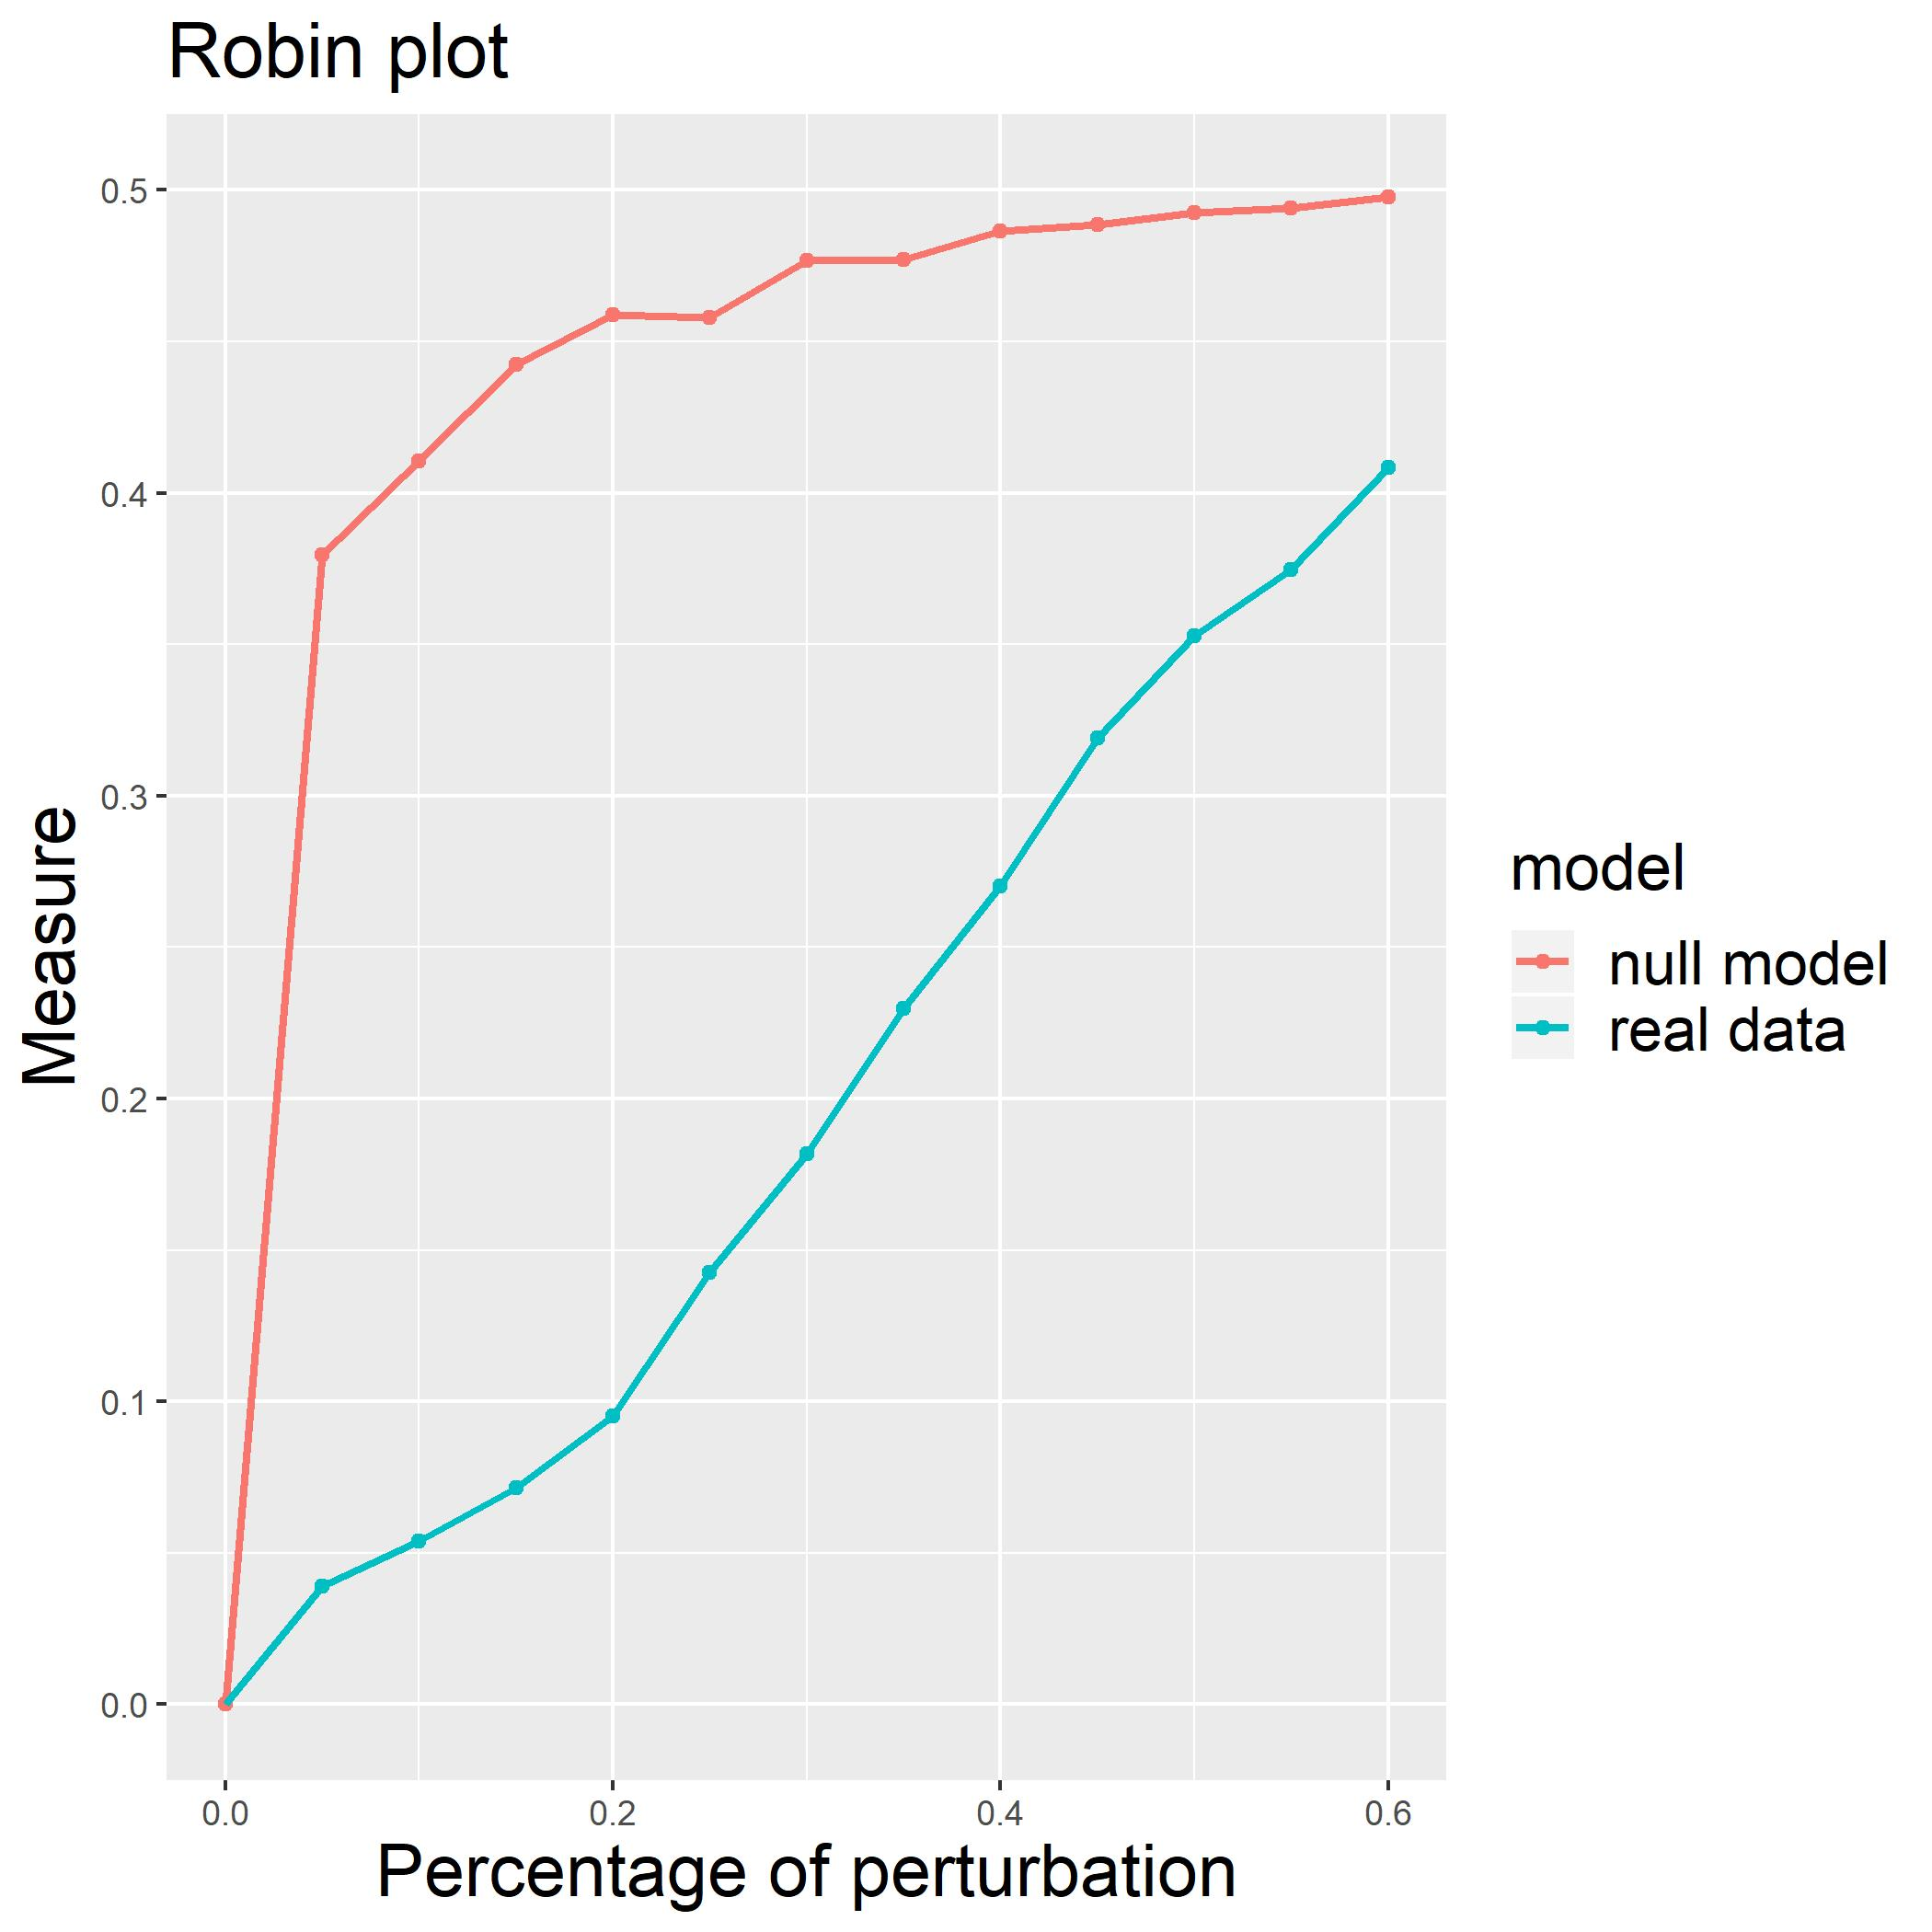
\includegraphics[width=.4\textwidth, height=5cm]{PlotRobin.png}
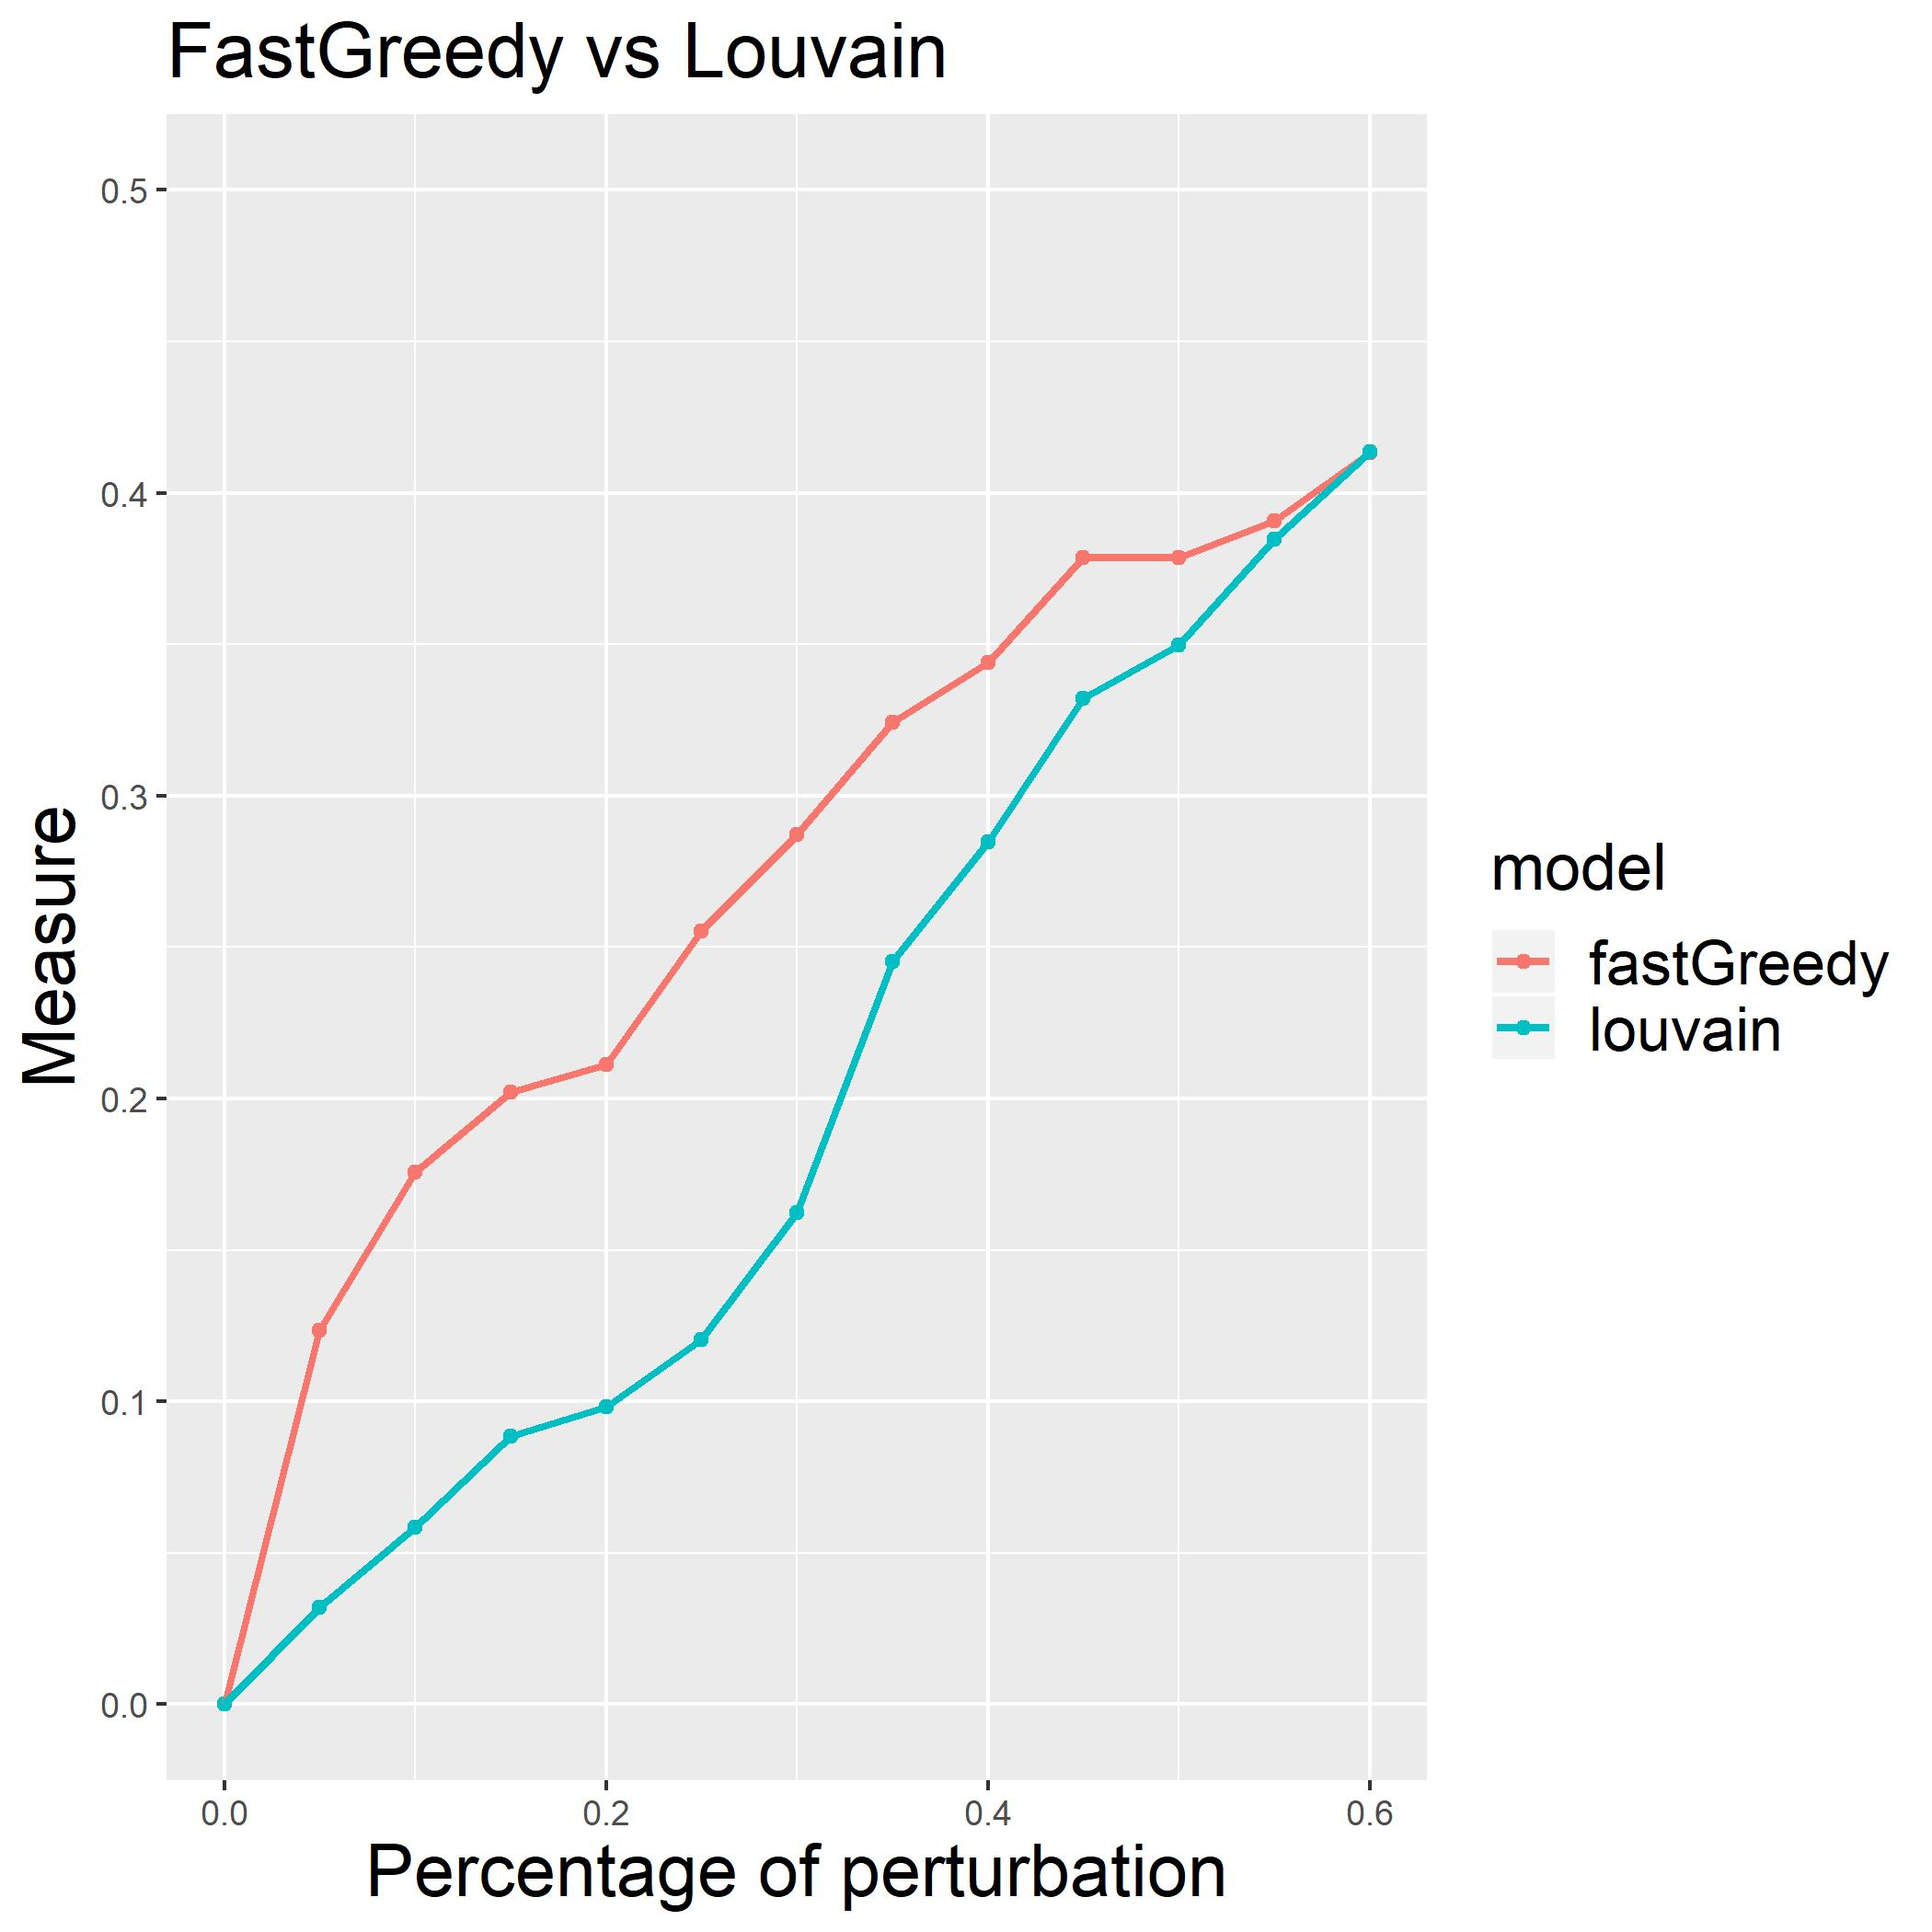
\includegraphics[width=.4\textwidth, height=5cm]{PlotCompare.png}
\caption{Curves of the null model and the real data generated by the VI stability measure and the Louvain detection algorithm on the American College Football network (Left panel). Curves of the Louvain and Fast greedy algorithm generated by the VI stability measure on the American College Football network (Right panel) \citep{GirvanNewman:2002}.}
\label{fig:PlotComparison}
\end{figure}

\subsection{Testing}
The GP test is implemented in \code{robinGPTest} and uses the R package \pkg{gprege} \citep{KalaitzisLawrence2011}. The ITP test is implemented in \code{robinFDATest} and uses the R package \pkg{fdatest} \citep{PiniVantini:2015}. The area under the curves is calculated by the function \code{robinAUC} and relies on the \pkg{DescTools} package. Figure \ref{fig:PlotComparisonFDA} shows the curves for the comparison of Louvain and Fast greedy algorithms' performance generated by the VI stability measure using the Interval Testing Procedure on the American College Football network (left panel) \citep{GirvanNewman:2002} and corresponding adjusted \textbf{\emph{p}}-values (right panel).

\begin{figure}[h]
\centering
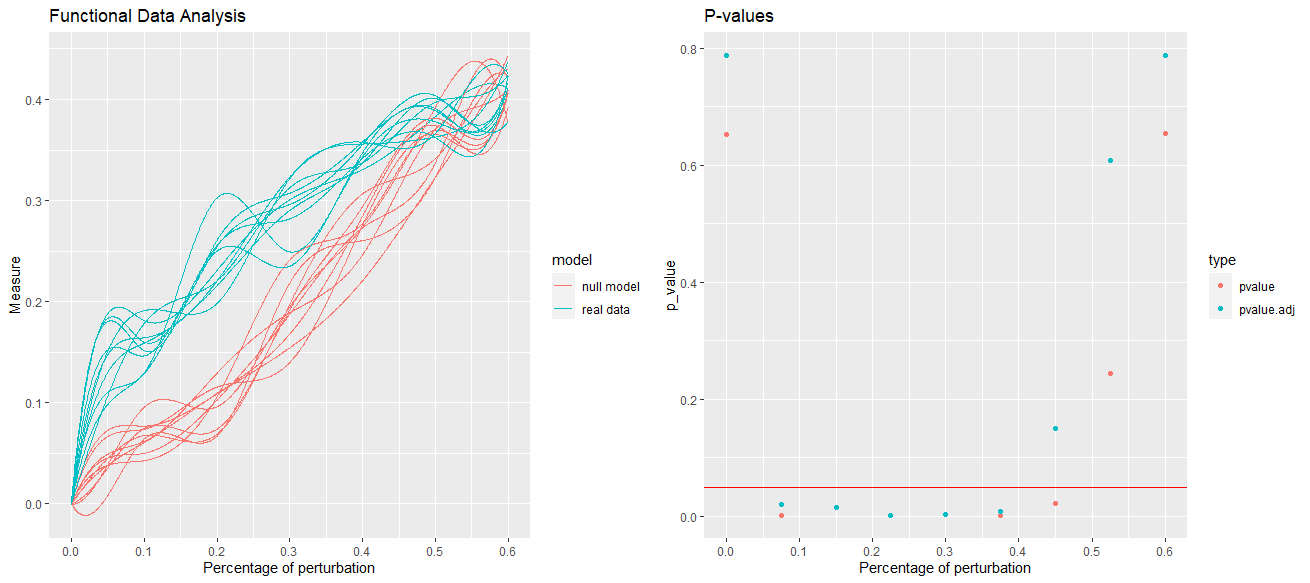
\includegraphics[width=.9\textwidth, height=6cm]{FDA.png}


\caption{Curves of the Louvain and Fast greedy algorithm generated by the VI stability measure using the Interval Testing Procedure on the American College Football network (Left panel). Corresponding p-values and adjusted p-values for all the intervals with the horizontal red line on to the critical value 0.05 (Right panel).}
\label{fig:PlotComparisonFDA}
\end{figure}

All the functions implemented in \pkg{robin} are summarized in Table \ref{tab-functions}.


\begin{table}[!h]
\centering
\caption{Summary of the functions implemented in \pkg{robin}.}
\label{tab-functions}
\begin{tabularx}{\textwidth}{l|X} 
\hline
\sc{Function} & \sc{Description} \\ \hline
\bf{Import/Manipulation} & \\
\\
\code{prepGraph} & Management and preprocessing \newline of input graph \\
\\
\code{random} & Building of null model  \\
\\
\hline
\bf{Analysis} & \\ 
\\
\code{robinRobust} & Comparison of a community detection method \newline versus random perturbations of the original graph\\
\\
\code{robinCompare} & Comparison of two different \newline community detection methods\\
\\
\hline
\bf{Visualization} & \\ 
\\
\code{methodCommunity} & Detection of the community structure   \\
\\
\code{membershipCommunities} & Detection of the membership vector \newline of the community structure  \\
\\
\code{plotGraph} & Graphical interactive representation \newline of the network  \\
\\
\code{plotComm} & Graphical interactive representation \newline of the network and its communities  \\
\\
\code{plotRobin} & Plots of the two curves \\
\\
\hline
\bf{Test} & \\ 
\\
\code{robinGPTest} & GP test and evaluation of the Bayes factor  \\
\\
\code{robinFDATest} & ITP test and evaluation of the adjusted p-values \\
\\
\code{robinAUC} & Evaluation of the area under the curve  \\
\hline
\end{tabularx}
\end{table}


\subsection{Computational time}	
The time complexity of the proposed strategy, more precisely of the \code{robinRobust} function, is evaluated as follows. Generating a rewired network with $N$ nodes and $M$ edges consumes $O(N+M)$ time, for both the real and the null model. For each network, we detect the communities, using any community detection algorithm present in \pkg{igraph} or any custom external algorithm inserted by the user, and calculate a stability measure. Let D be the time complexity associated with the community detection algorithm chosen. The overall procedure is iterated $k=100$ times for each percentage $p$ of the $n_p=12$ perturbation levels ($p \in [0,p_{max}]$, $p_{max}=0.6$).
In total, the proposed procedure requires $O(D+(((N+M+D)*k)*n_p))$ time both for the real and the null model.

 In Table \ref{tab-Time}, we show the computational time evaluated on a computer with an Intel 4 GHz i7-4790K processor and 24GB of memory. In this example, we used $Louvain$ as a detection algorithm on the $LFR$ benchmark graphs \citep{Lancichinetti_2008}.
The time complexity could be mitigated using parallel computing, but this is not yet implemented.

\begin{table}[h!]
\centering
\caption{Computational time}
\label{tab-Time}
\begin{tabular}{l|l|l} 
\hline
\sc{Nodes} & \sc{Edges} & \sc{Time(secs)} \\ \hline
\code{100} & 500	& 2.1\\
\code{1000} & 9267	& 36.1\\
\code{10000} & 100024	& 361.8\\
\code{100000} & 994053	& 9411.6\\
\code{1000000} & 8105913	& 110981.5
\\
\hline
\end{tabular}
\end{table}







\section{Example test: the American College football network} \zlabel{sec:example}		

\pkg{robin} includes the {\it American College football} benchmark dataset as an analysis example that is freely available at \url{http://www-personal.umich.edu/~mejn/netdata/}.
The dataset contains the network of United States football games between Division I colleges during the 2000 season \citep{GirvanNewman:2002}. 
It is a network of 115 vertices that represent teams (identified by their college names) and 613 edges that represent regular-season games between the two teams they connect. 
The graph has the ground truth, where each node has a value that indicates to which of the 12 conferences it belongs, and this offers a good opportunity to test the ability of \pkg{robin} to validate the community robustness.
It is known that each conference contains around 8-12 teams. The games are more frequent between members of the same conference than between members of different conferences. They are on average seven between teams of the same conference and four between different ones.   
We applied all the methods listed in subsection \textbf{\ztitleref{sec:procedures}} to this network,  choosing as measure the VI metric. 


\begin{example}
library(robin)

my_network <- system.file("example/football.gml", package="robin")
graph <- prepGraph(file=my_network, file.format="gml")

attributes <- vertex_attr(graph, index = V(graph))
real <- attributes$value
real <- as_membership(real)

set.seed(10)
members_In <- membershipCommunities(graph=graph, method=DA)
VI_In <- compare(real, members_In, method="vi")

\end{example}


Note that the variable $DA$ refers to the detection algorithms present in \pkg{igraph} and can assume the following values: \textit{fastGreedy}, \textit{infomap}, \textit{walktrap}, \textit{edgeBetweenness}, \textit{spinglass}, \textit{leadingEigen}, \textit{labelProp}, \textit{louvain}. The function \code{compare} is contained in the package \pkg{igraph} and permits the assessment of the distance between two community structures according to the chosen method.

Table \ref{tab-VIresults} summarizes the VI results calculated between the real communities and the ones that the detection algorithms created.

\begin{table}[h]
\centering
\caption{VI measure between different methods and ground-truth.}
\label{tab-VIresults}
\begin{tabular}{l|l} 
\hline
\sc{Methods} & \sc{Normalized VI} \\ \hline
\code{cluster\_infomap} & 0.054\\
\code{cluster\_spinglass } & 0.063\\
\code{cluster\_louvain } & 0.076\\
\code{cluster\_label\_prop} & 0.076\\
\code{cluster\_walktrap} & 0.078\\
\code{cluster\_edge\_betweenness} & 0.083\\
\code{cluster\_fast\_greedy} & 0.185\\
\code{cluster\_leading\_eigen} & 0.196\\
\hline
\end{tabular}
\end{table}
 
It is possible to observe that the best performance is offered by Infomap, having the lowest VI value, followed by Spinglass. Louvain, Propagating Labels, Walktrap, and Edge betweenness have a similar intermediate VI value, 
while the worst performance is given by Fast greedy and Leading eigenvector. Then, we used \pkg{robin} to check if the results are confirmed by looking at the VI curves and the results of the testing procedure for the second workflow, i.e., the one comparing two detection algorithms, considering Infomap versus all the others. 

\begin{example}

comp <- robinCompare(graph=graph, method1=DA1,
                     method2=DA2, measure="vi", type="independent")

plotRobin(graph=graph, model1=comp$Mean1, model2=comp$Mean2,                  
          measure="vi")



\end{example}


Figure \ref{fig:PlotComparison_allInfomap} shows the results we obtained. If we focus on the perturbation interval $[0,0.3]$, it is possible to note the similar behavior between the curves representing Infomap/Spinglass, Infomap/Louvain, Infomap/Propagating Labels, Infomap/Walktrap, and Infomap/Edge betweenness, with a closer distance between Infomap/Spinglass. On the contrary, the curves Infomap/Fast greedy and Infomap/Leading eigenvector have an opposite behavior, building almost an ellipse. 
This confirms what is displayed in Table \ref{tab-VIresults}.



\begin{figure}[h]
\centering
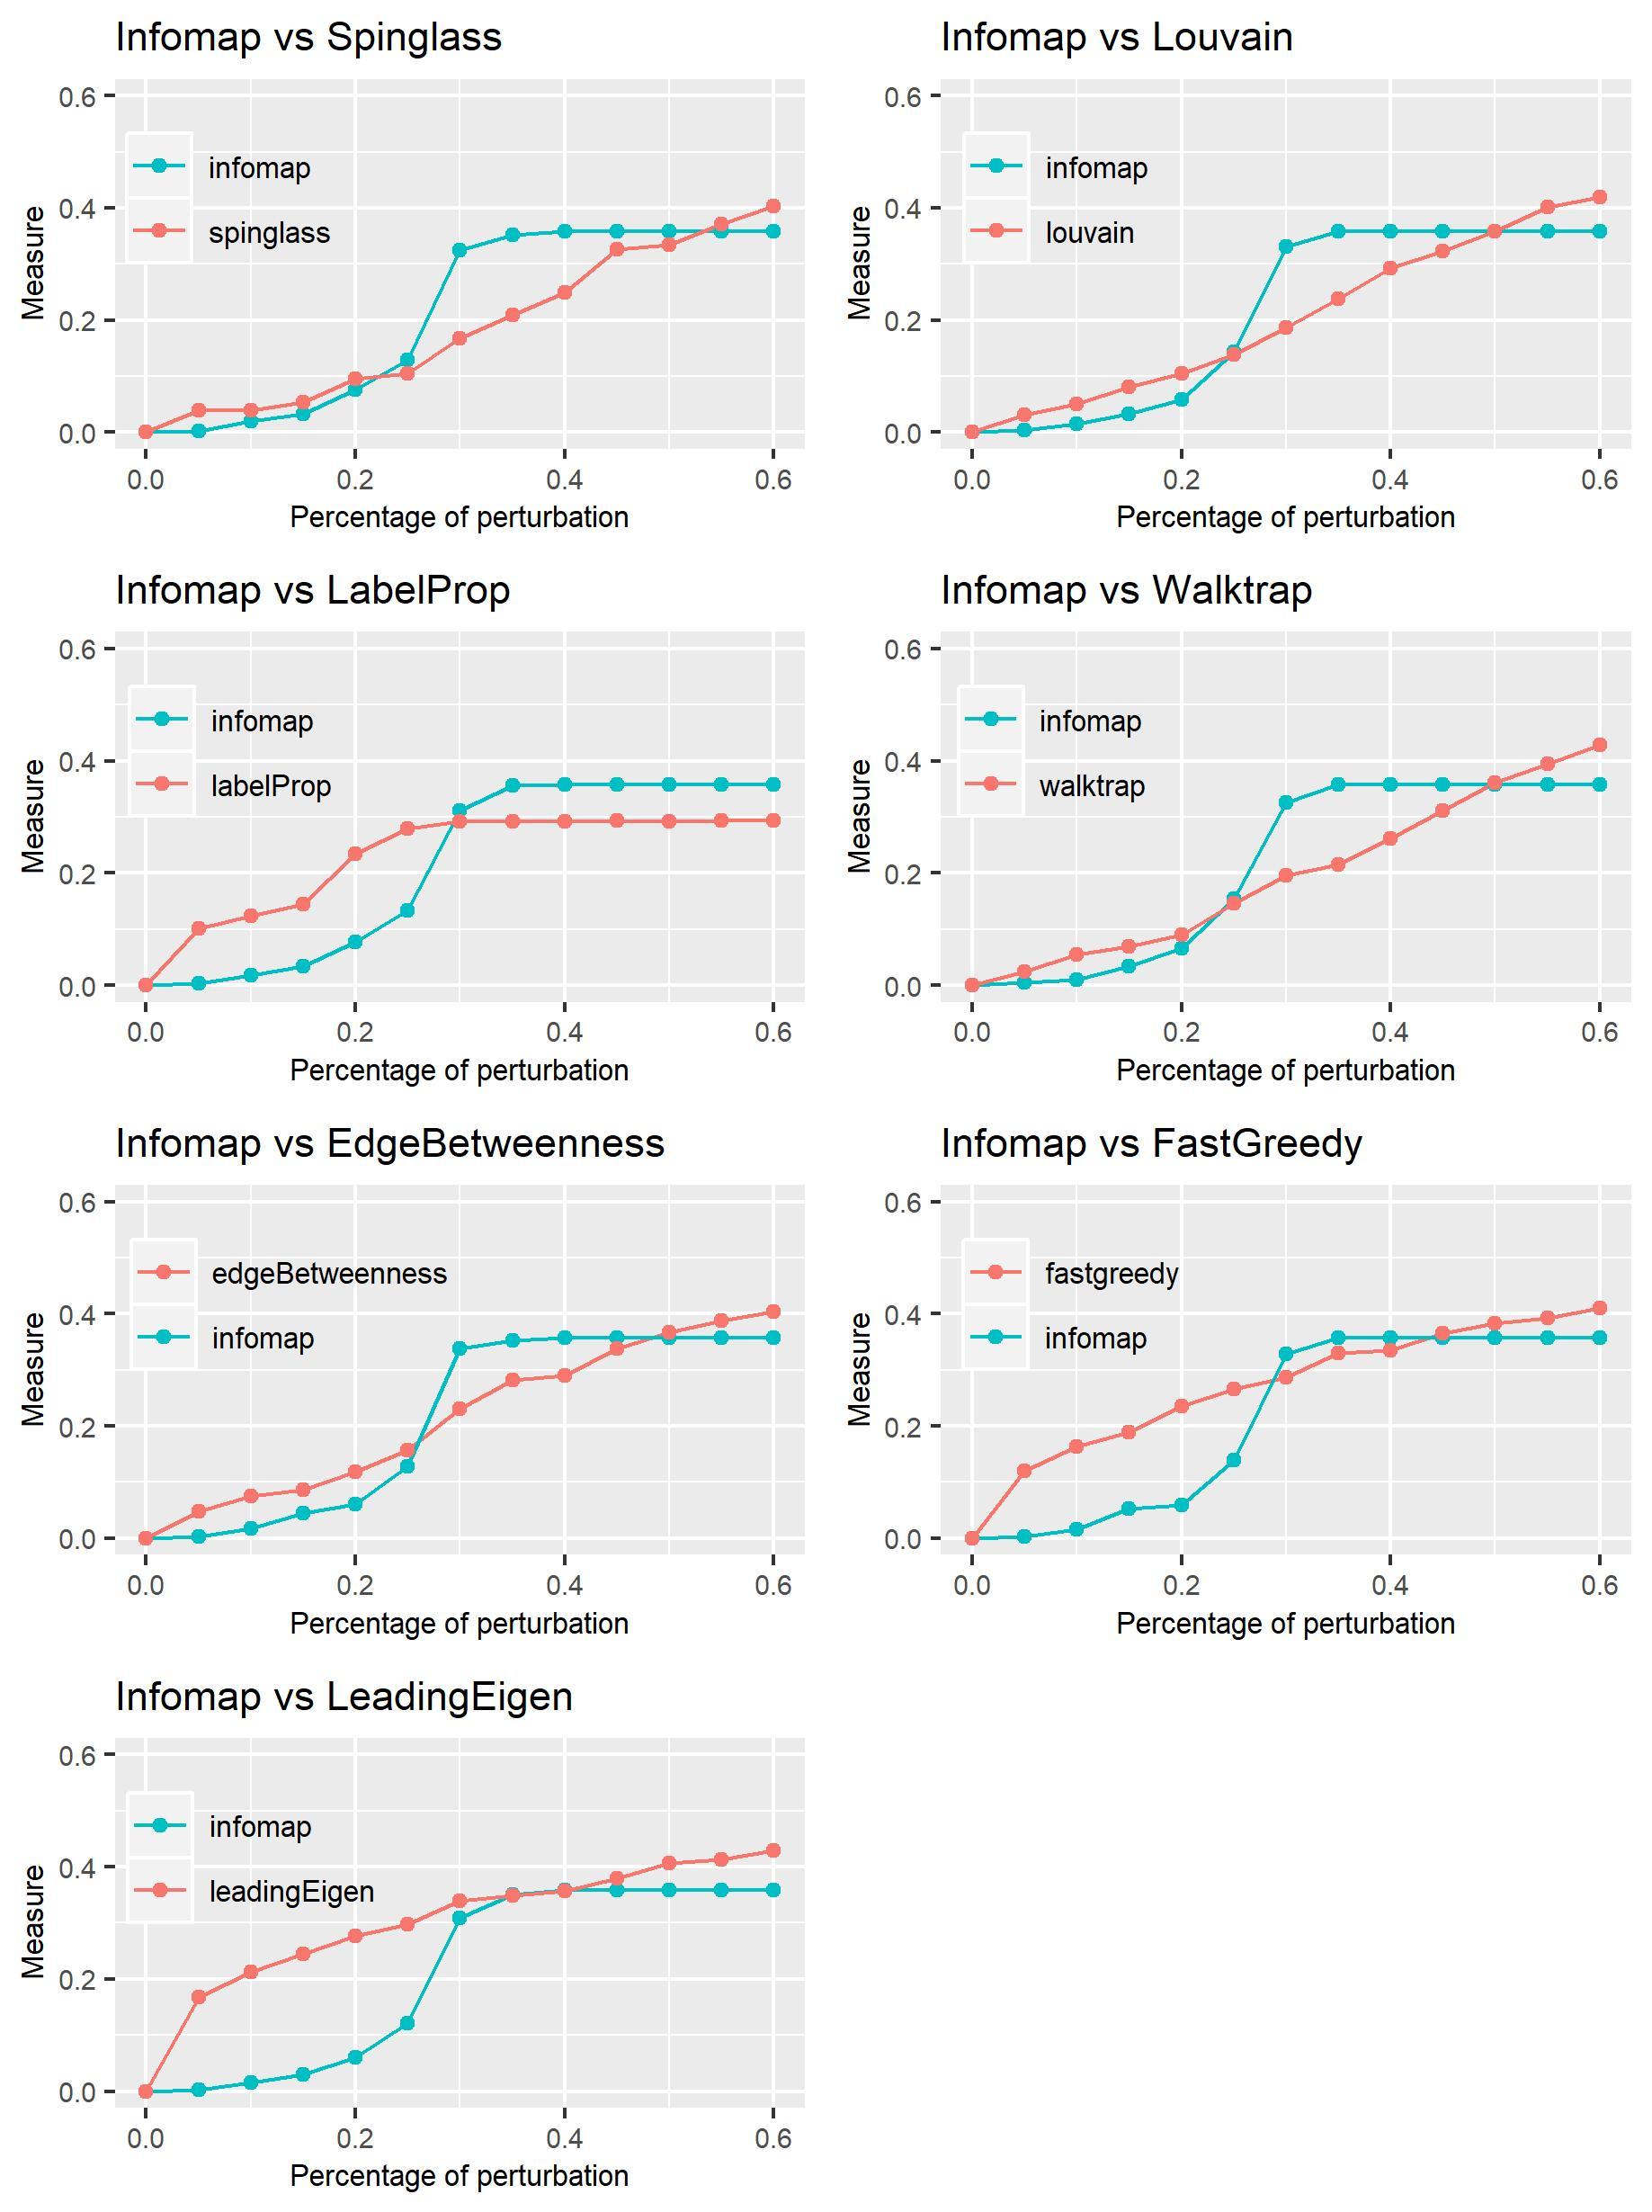
\includegraphics[width=14cm]{PlotComparisonAllVsInfomap.png}
\caption{Plot of the VI curves of Infomap against all other methods.}
\label{fig:PlotComparison_allInfomap}
\end{figure}



In our overall procedure, we explored two different ways of generating a null model, namely the Configuration Model (CM) and the {\it dk}-series model.

\begin{example}

graphRandomCM <- random(graph=graph)
graphRandomDK <- prepGraph(file="dk2.1_footballEdgelist.txt",
                          file.format = "edgelist")
                             
plotGraph(graph)
plotGraph(graphRandomCM)
plotGraph(graphRandomDK)

\end{example}

The different structures provided by the real data network, CM, and {\it dk}-series with $d=2.1$ are shown in Figure \ref{fig:PlotGraph}.  

\begin{figure}[h!]
\centering
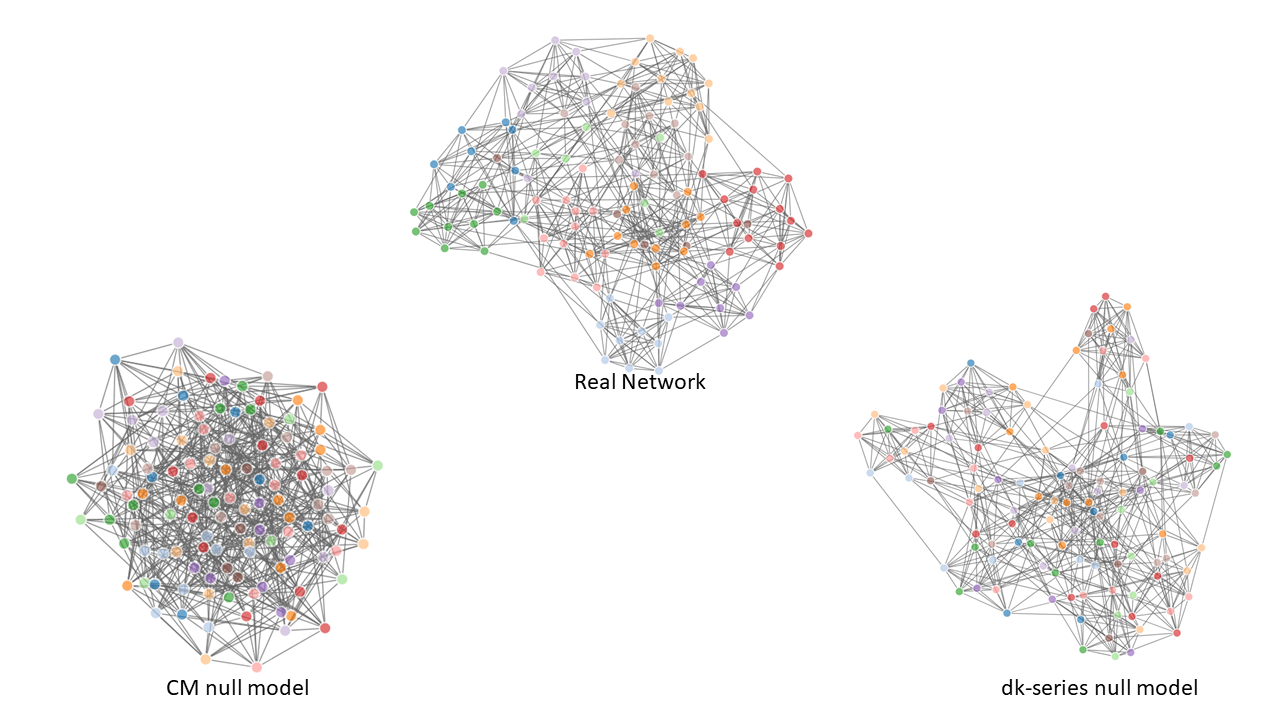
\includegraphics[width=14cm]{network.png}
\caption{Graph of the real data (Upper panel); graph of the CM null model (Left - lower panel); graph of the $dk$-series null model with $d=2.1$ (Right - lower panel).}
\label{fig:PlotGraph}
\end{figure}

The CM generates a random graph with the same degree sequence as the original one but with a randomized group structure. 
Our experiments show that CM is not a good null model when using Propagating Labels and Infomap as community extraction methods (Figure \ref{fig:PlotConfigurationModel}). 
In fact, when the modularity is low, these two algorithms tend to assign all the nodes to the same community, hence resulting in a flat stability measure curve. We launched the function \code{robinRobust}  to assess the robustness of each detection algorithm.  

\begin{example}

proc_CM <- robinRobust(graph=graph, graphRandom=graphRandomCM,
                       measure="vi", method=DA, type="independent")

plotRobin(graph=graph, model1=proc_CM$Mean,model2=proc_CM$MeanRandom,
          measure="vi") 
\end{example}
 
\begin{figure}[h]
\centering
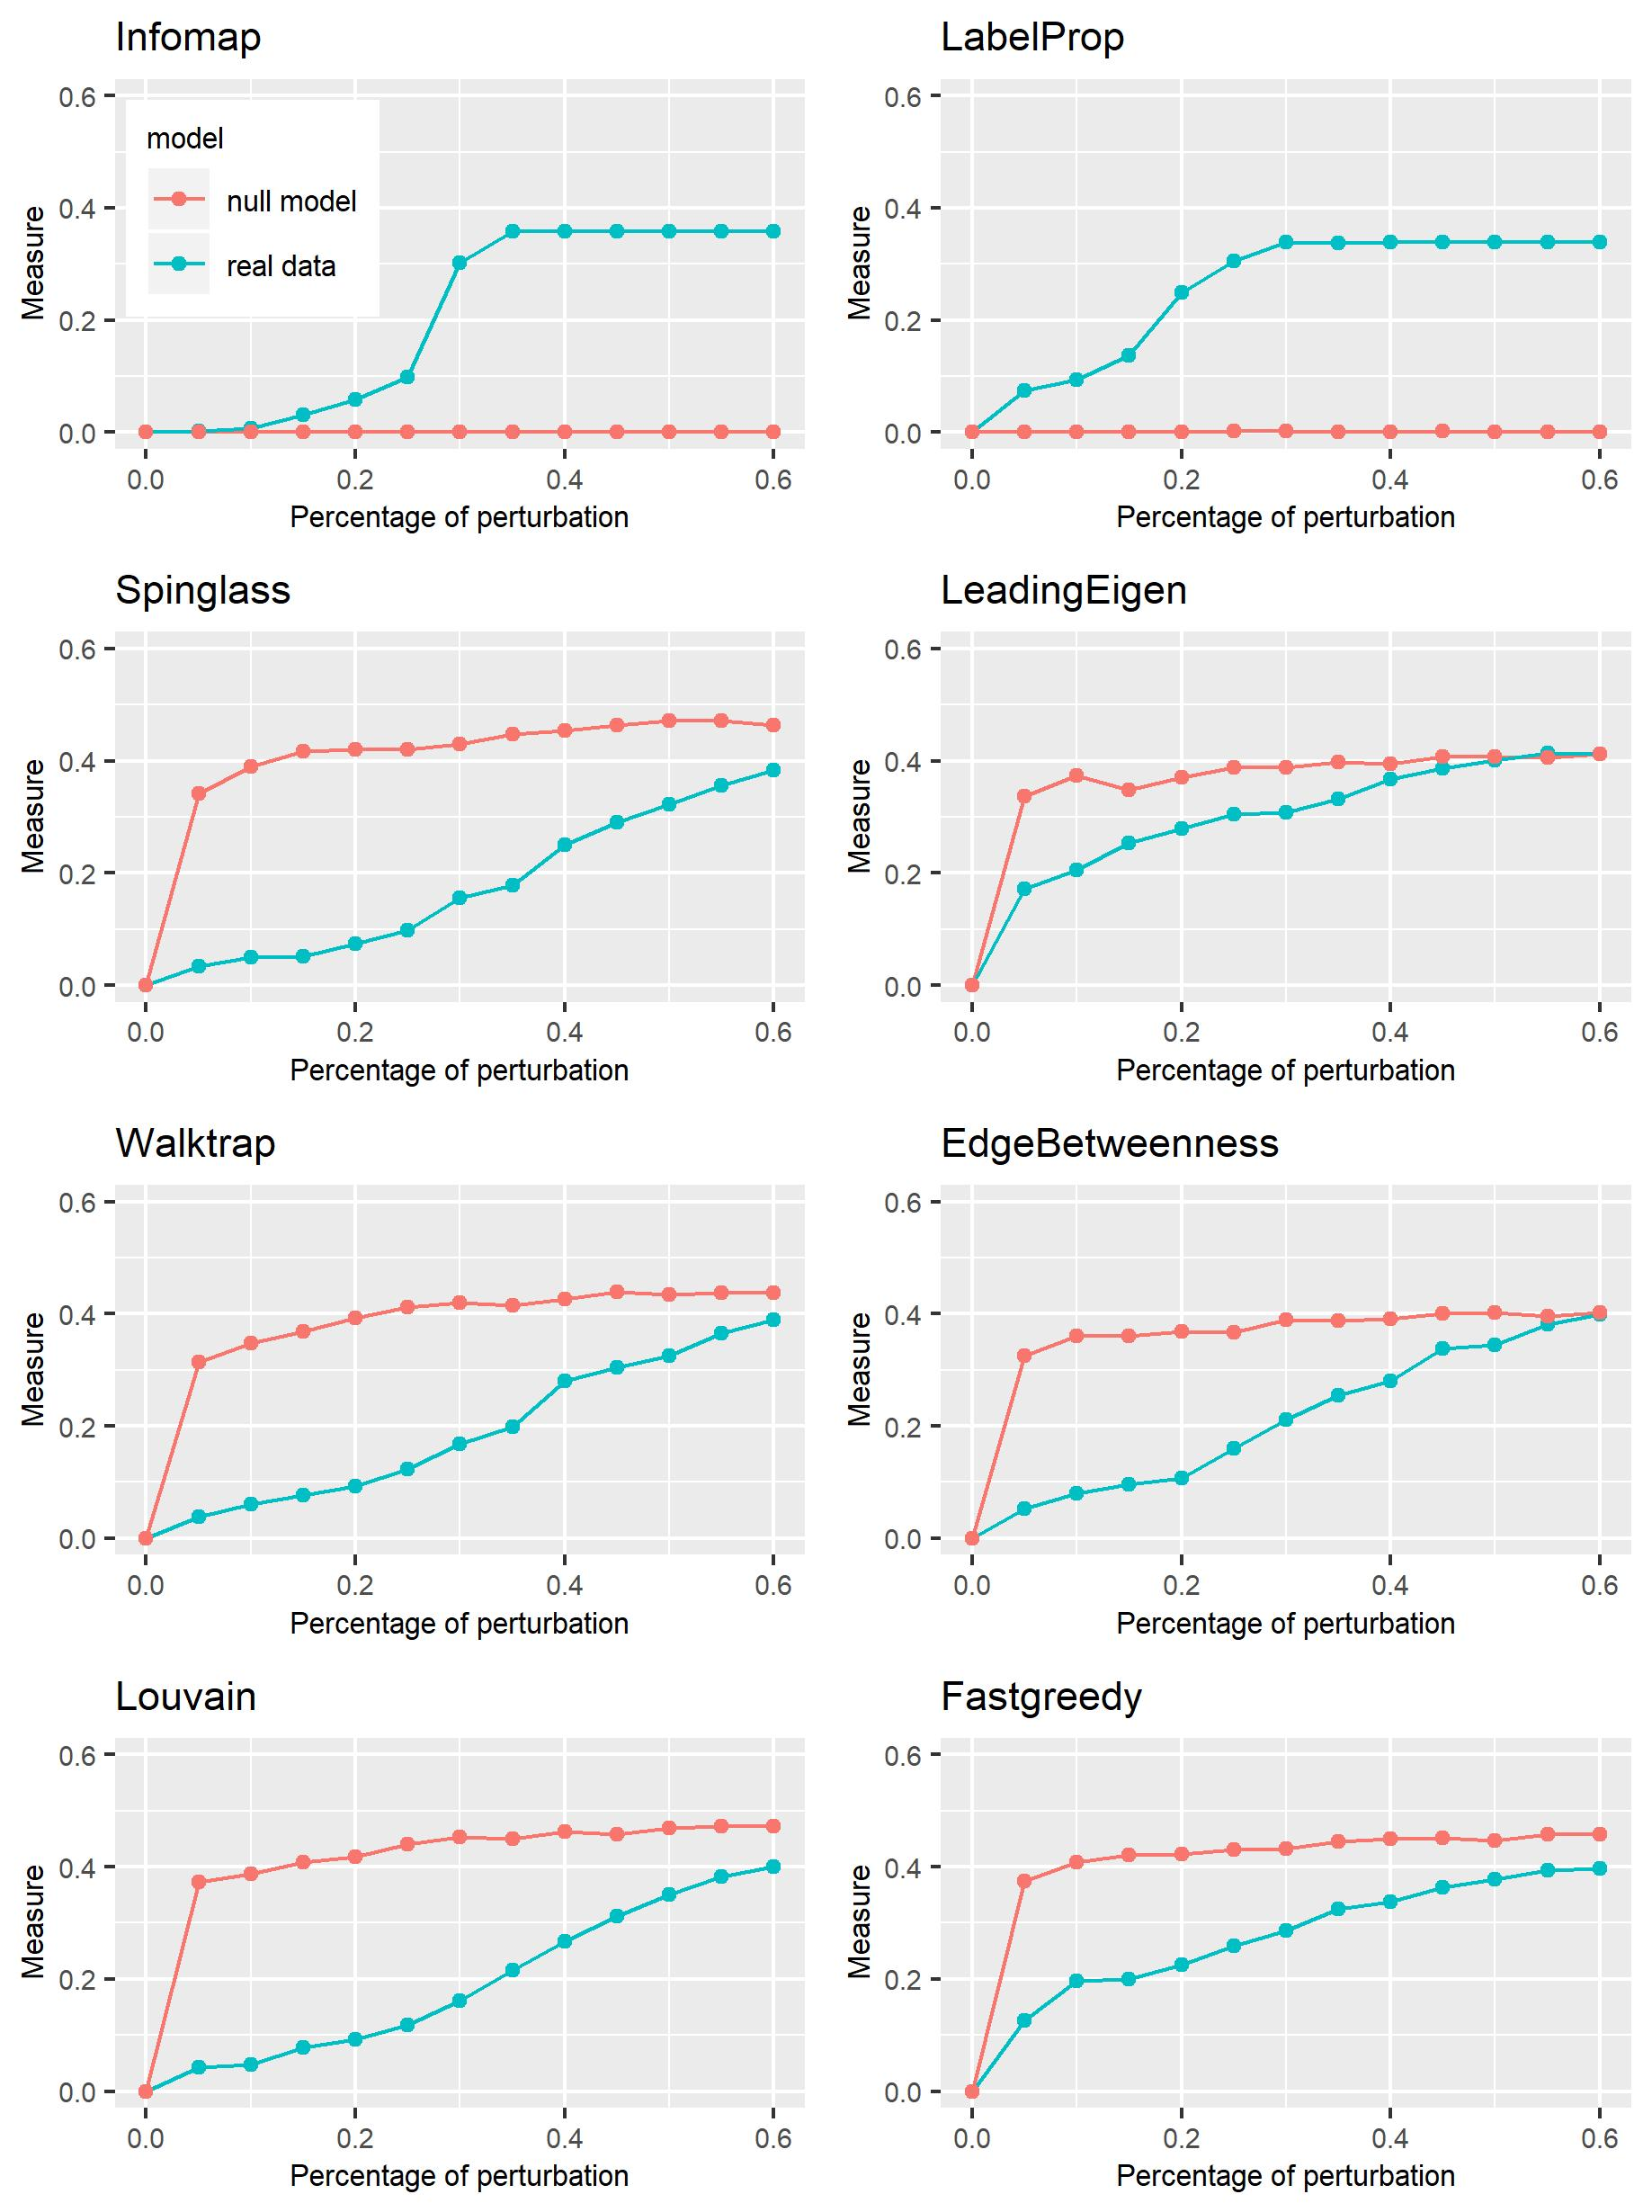
\includegraphics[width=14cm]{PlotConfigurationModel.png}
\caption{Plot of the VI curves of the CM null model and all the algorithms implemented.}
\label{fig:PlotConfigurationModel}
\end{figure}


The {\it dk}-series model generates a random graph preserving the global organization of the original network at various increasing levels of details chosen by the user via the setting of the parameter $d$. In particular, we chose the {\it dk} random graph with d=2.1. 

\begin{example}
proc_DK <- robinRobust(graph=graph, graphRandom=graphRandomDK, 
                       measure="vi", method="fastGreedy", type="independent")
                  
plotRobin(graph=graph, model1=proc_DK$Mean, model2=proc_DK$MeanRandom,
          measure="vi")

\end{example}

Figure \ref{fig:PlotDkModel} shows the stability measure curves of each detection algorithm compared to dk 2.1 null model. For all the methods, the two curves are very close due to the capability of the null model to preserve a structure similar to the real network and visually confirm the results in Table \ref{tab-VIresults}.
\begin{figure}[h!]
\centering
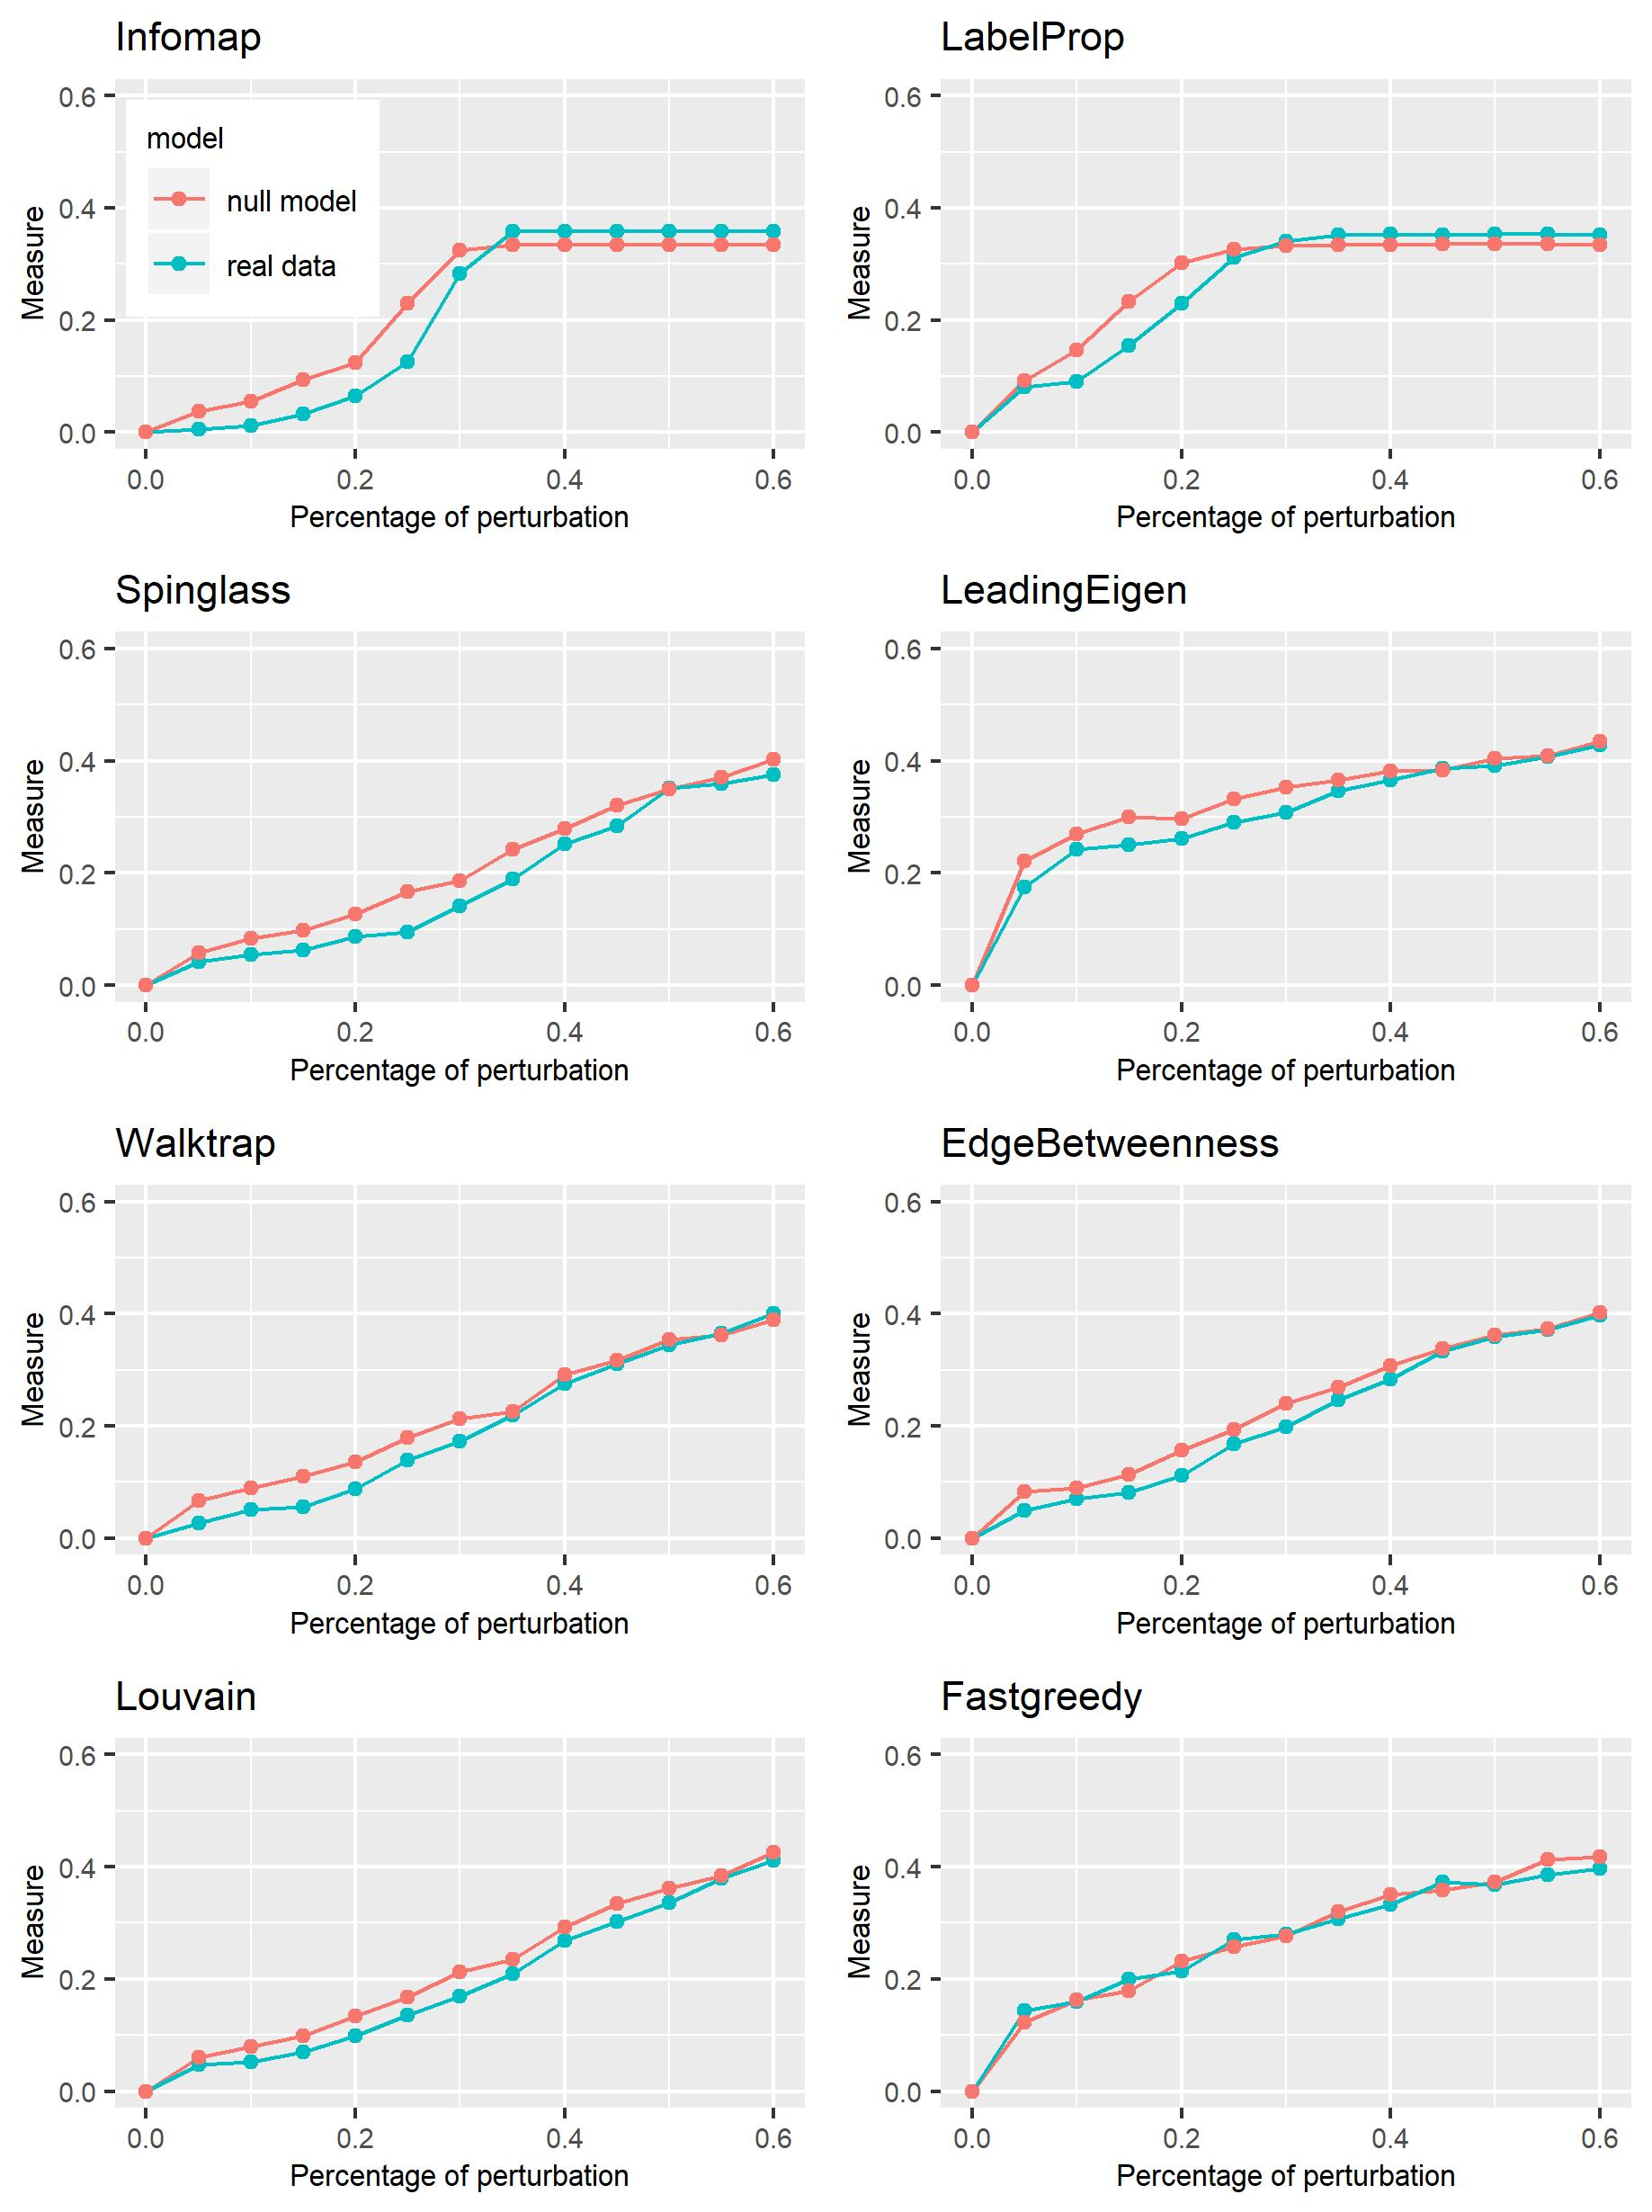
\includegraphics[width=14cm]{PlotDkModel.png}
\caption{Plot of the VI curves of the  {\it dk}-series null model with $d=2.1$ and all the algorithms implemented.}
\label{fig:PlotDkModel}
\end{figure}

Moreover, for the {\it dk}-series model, we tested the differences between the two curves using the GP methodology implemented in the function in \code{robinGPTest}.

\begin{example}

BFdk <- robinGPTest(model1=proc_DK$Mean, model2=proc_DK$MeanRandom)

\end{example}
The results are shown in Table \ref{tab-BayesAIC} and agree with those shown in Table \ref{tab-VIresults}. 

\begin{table}[h!]
\centering
\caption{Bayes Factor and AUC ratio for {\it dk} -series with $d=2.1$}
\label{tab-BayesAIC}
\begin{tabular}{l|l|l} 
\hline
\sc{Methods} & \sc{Bayes Factor} & AUC \\ \hline
\code{cluster\_infomap} & 53.67	& 1.133\\
\code{cluster\_spinglass } & 40.55	& 1.249\\
\code{cluster\_louvain } & 31.52	& 1.208\\
\code{cluster\_label\_prop} & 102.2	& 0.852\\
\code{cluster\_walktrap} & 30.74	& 1.204\\
\code{cluster\_edge\_betweenness} & 31.10	& 1.194\\
\code{cluster\_fast\_greedy} & 0.001 & 1.017\\
\code{cluster\_leading\_eigen} & 8.474	& 1.042\\
\hline
\end{tabular}
\end{table}

Fastgreedy clearly fails in recovering the communities. LeadingEigen has stronger evidence but too weak when compared to the other methods. 
Louvain, Walktrap, and EdgeBetweenness have the same strong evidence followed by Spinglass and Infomap. 
LabelProp shows the strongest evidence, but the result is obviously influenced by the swap between the two curves when the perturbation is greater than 20$\%$, underlying a worse performance of the algorithm. 
The same swap can be noted for Infomap at 35$\%$ perturbation level, but with less difference between the two curves.
This is confirmed by the fact that the ratios between the AUC of the real null model curve and the AUC of the real network are close to 1. 

\begin{example}

AUC <- robinAUC(graph=graph, model1=proc_DK$Mean,
                model2=proc_DK$MeanRandom, measure="vi")
AUCdkratio <- AUC$area2/AUC$area1

\end{example}



 
Also, note that LabelProp originates the paradox that the AUC of the real model curve exceeds the AUC of the null network, despite the hypothesis testing result is positive. Hence, it is always the case to look at the plots and AUC ratios. 


\section{Conclusion} \label{sec:Conclusion}
In this paper, we presented \pkg{robin}, an R/CRAN package, to assess the robustness of the community structure of a network found by one or more detection methods, providing an indication of their reliability. The procedure implemented is useful for comparing different community detection algorithms and choosing the one that best fits the network of interest. More precisely, \pkg{robin} initially detects if the community structure found by some algorithms is statistically significant, then it compares the different selected detection algorithms on the same network. \pkg{robin} uses analysis tools set up for functional data analysis, such as $GP$ regression and $ITP$. The core functions of the package are \code{robinRobust} and \code{robinCompare}, which build the stability measure curves for the null model and the network understudy for a fixed detection algorithm and the stability measure for the network understudy for two detection algorithms, respectively. Moreover, \code{robinGPTest} and \code{robinFDATest} implement the GP test and the ITP test. We illustrated the usage of the package on a benchmark dataset. The package is available on CRAN at \url{https://CRAN.R-project.org/package=robin}.


%% -- Optional special unnumbered sections -------------------------------------

\section{Computational details}

The results in this paper were obtained using R~3.6.1 with the packages \pkg{igraph} version 1.2.4.2,  \pkg{networkD3} version 0.4, \pkg{ggplot2} version 3.2.1,  \pkg{gridExtra} version 2.3,  \pkg{fdatest} version 2.1, \pkg{gprege} version 1.30.0, and \pkg{DescTools} version 0.99.31. R itself and all packages used are available from the Comprehensive R Archive Network (CRAN) at \url{https://CRAN.R-project.org/}.


\section{Acknowledgements}

This work was supported by the project Piattaforma Tecnologica ADVISE - Regione Campania, by the project “TAILOR” (H2020-ICT-48 GA: 952215) and by DiSTABiF at the University of Campania Luigi Vanvitelli that is coordinating V.P. PhD program. 

\section{Contributions}
V.P. implemented the software and analyzed its properties. 
D.R. supported V.P. in R package implementation.
A.C., L.C., and I.D.F. conceived the work, equally contributed to the development and implementation of the concept, discussed and analyzed the results. 
A.C., L.C., I.D.F., and V.P. wrote the manuscript.


\bibliography{policastro}


\address{Valeria Policastro ({\it package author and creator})\\
  Dipartimento Scienze e Tecnologie Ambientali, Biologiche e Farmaceutiche\\
  Universit\'a degli Studi della Campania ``Luigi Vanvitelli'' \\
  Via Vivaldi, 43  
  81100 Caserta, Italia\\
  and\\
  Istituto per le Applicazioni del Calcolo ``M. Picone'' - sede di Napoli\\
  Consiglio Nazionale delle Ricerche\\
  via Pietro Castellino 111\\
  80131 Napoli, Italy\\
  \email{valeria.policastro@unicampania.it}}

\address{Dario Righelli \\
  Dipartimento di Statistica\\
  Universit\'a di Padova \\
  Via Cesare Battisti, 241  
  35121 Padova, Italia\\
  and\\
  Istituto per le Applicazioni del Calcolo ``M. Picone'' - sede di Napoli\\
  Consiglio Nazionale delle Ricerche\\
  via Pietro Castellino 111\\
  80131 Napoli, Italy\\
 \email{d.righelli@na.iac.cnr.it}}
  
\address{Annamaria Carissimo \\
  Istituto per le Applicazioni del Calcolo ``M. Picone'' - sede di Napoli\\
  Consiglio Nazionale delle Ricerche\\
  via Pietro Castellino 111\\
  80131 Napoli, Italy\\
  \textit{Co-last and corresponding author}\\
  \email{a.carissimo@iac.cnr.it}}
  
\address{Luisa Cutillo \\
  School of Mathematics\\
  University of Leeds\\
  Leeds\\
  LS2 9JT, United Kingdom\\
   and\\
  Dipartimento di Studi Aziendali e Quantitativi\\
  Universit\'a degli Studi di Napoli ``Parthenope' \\
  Via Generale Parisi, 13 \\ 
  80132, Napoli, Italia\\
  \textit{Co-last and corresponding author}\\
  \email{l.cutillo@leeds.ac.uk}}
 
\address{Italia De Feis \\
  Istituto per le Applicazioni del Calcolo ``M. Picone'' - sede di Napoli\\
  Consiglio Nazionale delle Ricerche\\
  via Pietro Castellino 111 \\
  80131 Napoli, Italy\\
  \textit{Co-last and corresponding author}\\
\email{i.defeis@iac.cnr.it}}






